\documentclass[11pt,a4paper]{article}

% ---------- packages ----------
\usepackage[margin=2.4cm]{geometry}
\usepackage{times}
\usepackage{amsmath,amssymb,amsfonts}
\usepackage{booktabs}
\usepackage{tabularx}
\usepackage{multirow}
\usepackage{graphicx}
\usepackage{subcaption}
\usepackage{float}
\usepackage{xcolor}
\usepackage{hyperref}
\usepackage{enumitem}
\usepackage{setspace}
\usepackage{microtype}
\usepackage{caption}
\usepackage{array}
\usepackage{makecell}

\hypersetup{
  colorlinks=true,
  linkcolor=black,
  citecolor=black,
  urlcolor=blue
}

\captionsetup{font=small,labelfont=bf}
\onehalfspacing
\graphicspath{{figures/}}

\title{
\vspace{-1.2em}
\textbf{An Empirical Reproduction and Analysis of Auditory Filter Model Frontends for Speaker Gender Recognition}\\[0.6em]
\large Implementation Report
}
\author{
  Reproduction of Fayyazi \& Shekofteh (2023)\\[0.3em]
  \normalsize\textit{Applied Acoustics}, Vol.~213, Art.~109635
}
\date{\today}

\begin{document}
\maketitle

\begin{abstract}
\noindent
This report presents a systematic, end-to-end reproduction of the auditory filter model (AFM) convolutional frontend framework for binary speaker gender recognition proposed by Fayyazi and Shekofteh (2023). We implement eight first-layer frontends---Free-CNN, Mel-CNN, Sinc, Sinc2, Gamma, Gauss, Cascade, and a mean-shift--pruned Reduced bank---within a SincNet-style architecture operating on raw 16\,kHz waveforms. Models are trained on TIMIT, fine-tuned on LibriSpeech, and evaluated for generalization on RAVDESS and VoxCeleb1-test. Quantitative results are compared against the published Tables~4, 7 and~8. On TIMIT, utterance accuracy typically lies within $\pm 0.5$ percentage points of the paper mean, with the Reduced and Sinc models attaining the lowest classification error rate (CER~$=0.67\%$). Out-of-domain performance on RAVDESS and VoxCeleb1-test remains competitive but falls short of the published figures. We attribute this gap to a shorter fine-tuning schedule (20 vs.\ 200 epochs), a substantially smaller fine-tuning corpus (LibriSpeech \texttt{dev-clean} vs.\ \texttt{train-clean-360}), evaluation on the VoxCeleb1 test partition only, and single-run rather than three-run reporting. Supporting visualizations---training curves, complex-plane pole reduction, accumulative magnitude responses, center-frequency histograms, quality-factor trajectories, and t-SNE embeddings---are included throughout.
\end{abstract}

\tableofcontents
\newpage

% ============================================================
\section{Introduction}
% ============================================================

Speaker gender recognition (SGR)---the binary classification of a talker as male or female from the acoustic signal---is a classical problem in speech processing with applications in diarization, human--computer interaction, and forensic analysis. Deep convolutional networks operating on raw waveforms have recently achieved strong accuracy, yet unconstrained first-layer filters are difficult to interpret and often over-parameterized relative to the physical structure of hearing.

Fayyazi and Shekofteh~\cite{fayyazi2023} address this limitation by replacing free convolutional kernels with parametric \emph{auditory filter models} (AFMs)---Sinc, Sinc2 (triangular), Gammatone, Gaussian, and Cascaded Gaussian---and by further pruning Cascade poles via mean-shift clustering to obtain a compact Reduced filter bank. Their pipeline comprises TIMIT training, LibriSpeech fine-tuning, and out-of-domain evaluation on VoxCeleb1 and RAVDESS, accompanied by interpretability analyses (magnitude responses, center-frequency distributions, quality factors, and feature embeddings).

The present work aims to:
\begin{enumerate}[leftmargin=1.6em,itemsep=0.25em]
  \item reproduce the architectural and training protocol of~\cite{fayyazi2023} as faithfully as computational constraints permit;
  \item report CER, frame error rate (FER), and utterance accuracy for all frontends on TIMIT, RAVDESS, and VoxCeleb1-test;
  \item quantify discrepancies with the published tables and provide a principled account of their causes;
  \item document training dynamics and filter-level analyses, including the complex-plane pole reduction that underlies the Reduced model.
\end{enumerate}

% ============================================================
\section{Method Overview}
% ============================================================

\subsection{Task definition and metrics}

Given a raw waveform $x$, the system predicts a gender label $y\in\{0,1\}$ (male/female). Audio is segmented into overlapping chunks of duration $T{=}200$\,ms with hop $H{=}10$\,ms after energy-based silence removal. Frame-level predictions are aggregated by majority vote to obtain an utterance-level decision. Following the paper, we report:
\begin{itemize}[leftmargin=1.6em,itemsep=0.2em]
  \item \textbf{FER:} fraction of misclassified 200\,ms frames;
  \item \textbf{CER:} fraction of misclassified utterances after majority voting;
  \item \textbf{Accuracy:} $100-\mathrm{CER}$ (\%).
\end{itemize}

\subsection{Network architecture}

The backbone matches the SincNet-style topology of~\cite{fayyazi2023}:
\begin{align*}
  x &\xrightarrow{\;\mathrm{Conv1}\;} \mathrm{Pool}_3 \to \mathrm{LN} \to \mathrm{LReLU}\\
    &\xrightarrow{\;\mathrm{Conv2}\;} \mathrm{Pool}_3 \to \mathrm{LN} \to \mathrm{LReLU}\\
    &\xrightarrow{\;\mathrm{Conv3}\;} \mathrm{Pool}_3 \to \mathrm{LN} \to \mathrm{LReLU}\\
    &\to \mathrm{Flatten} \to (\mathrm{FC}_{2048}+\mathrm{BN})\times 3 \to \mathrm{Softmax}_2.
\end{align*}
Conv1 comprises $N{=}80$ filters of length $L{=}257$ (except Reduced, where $N$ is determined by clustering). Conv2 and Conv3 each use 60 filters of kernel size 5. The loss is negative log-likelihood; the optimizer is RMSprop with learning rate $10^{-3}$ and batch size 128.

\subsection{Auditory filter model frontends}

\begin{table}[H]
\centering
\caption{First-layer frontends considered in this study.}
\label{tab:frontends}
\begin{tabular}{@{}llp{7.2cm}@{}}
\toprule
\textbf{Name} & \textbf{Type} & \textbf{Description} \\
\midrule
Free-CNN & Unconstrained & Fully learnable FIR kernels \\
Mel-CNN  & Fixed         & Frozen Mel-scaled filter bank \\
Sinc     & AFM           & Band-pass sinc (rectangular spectrum) \\
Sinc2    & AFM           & Squared-sinc / triangular spectrum \\
Gamma    & AFM           & Gammatone impulse response \\
Gauss    & AFM           & Gaussian band-pass \\
Cascade  & AFM           & Cascade of two Gaussians (two poles/filter) \\
Reduced  & Pruned        & Mean-shift centroids of Cascade poles $\to$ frozen triangular bank \\
\bottomrule
\end{tabular}
\end{table}

\subsection{Pole reduction (Reduced model)}

Following Sec.~3.2.2 of~\cite{fayyazi2023}, Cascade filters are mapped to complex poles
\begin{equation}
  a = e^{-B+j\,f_c},
\end{equation}
where $f_c$ and $B$ denote center frequency and bandwidth in radians per sample. Poles are clustered by mean-shift; cluster centers are converted back to $(f_c,B)$ and realized as triangular FIR filters. The resulting bank is frozen and the remaining layers are retrained. In our run, clustering retained \textbf{26} filters (paper target: $\approx 40$).

% ============================================================
\section{Experimental Pipeline}
% ============================================================

The reproduction proceeds in seven stages:

\begin{enumerate}[leftmargin=1.6em,itemsep=0.35em]
  \item \textbf{Preprocessing.} Silence removal (VAD) and resampling to 16\,kHz.
  \item \textbf{TIMIT training.} Each frontend is trained for 50 epochs on TIMIT (train/val/test $\approx$ 3700 / 920 / 1344 utterances after excluding SA sentences).
  \item \textbf{Filter analysis.} Accumulative magnitude response, center-frequency histogram, quality factor $Q=f_c/B$, and t-SNE of convolutional features.
  \item \textbf{Model reduction.} Cascade poles $\to$ mean-shift $\to$ Reduced bank $\to$ retrain on TIMIT (50 epochs, frozen Conv1).
  \item \textbf{Fine-tuning.} 20 epochs on LibriSpeech \texttt{dev-clean} (speaker-held-out validation); evaluate on \texttt{test-clean}.
  \item \textbf{Generalization.} Evaluation on RAVDESS (1440 utterances) and VoxCeleb1-test (4874 utterances).
  \item \textbf{Aggregation.} Comparison tables and figures against Tables~4, 7 and~8 of~\cite{fayyazi2023}.
\end{enumerate}

% ============================================================
\section{Training Configuration}
% ============================================================

Table~\ref{tab:hparams} contrasts the paper protocol with the settings used in this reproduction. Architecture, optimizer, learning rate, and batch size match the paper. The principal deviations---epoch budget, fine-tuning corpus, VoxCeleb evaluation set, and number of independent runs---are deliberate trade-offs driven by available compute and storage, and are revisited in Sec.~\ref{sec:discussion}.

\begin{table}[H]
\centering
\caption{Learning settings: paper vs.\ this work.}
\label{tab:hparams}
\begin{tabular}{@{}lll@{}}
\toprule
\textbf{Parameter} & \textbf{Paper} & \textbf{This work} \\
\midrule
Input                 & Raw waveform, 16\,kHz          & Identical \\
Chunk / hop           & 200\,ms / 10\,ms               & Eval: identical; train: 8 random chunks/utt/epoch \\
Silence removal       & Yes                            & Yes \\
Conv1                 & 80$\times$257                  & Identical (Reduced: 26) \\
Conv2 / Conv3         & 60, kernel 5, pool 3           & Identical \\
Classifier            & $3\times$FC\,2048 + BN         & Identical \\
Loss / optimizer      & NLL / RMSprop, $\mathrm{lr}{=}10^{-3}$ & Identical \\
Batch size            & 128                            & 128 \\
TIMIT epochs          & 500                            & \textbf{50} \\
Fine-tune epochs      & 200 on \texttt{train-clean-360}& \textbf{20} on \texttt{dev-clean} \\
Independent runs      & 3 (mean $\pm$ std)             & \textbf{1} (seed 42) \\
VoxCeleb evaluation   & Full VoxCeleb1 ($\approx$1251 spk) & VoxCeleb1-test ($\approx$40 spk) \\
\bottomrule
\end{tabular}
\end{table}

\paragraph{Training sampling note.}
Evaluation always uses the paper hop of 10\,ms for FER/CER. Exhaustive 10\,ms hopping over all frames at every training epoch is computationally prohibitive on a single laptop GPU; therefore training draws eight random 200\,ms chunks per utterance per epoch while preserving the chunk duration used in~\cite{fayyazi2023}.

% ============================================================
\section{Results}
% ============================================================

\subsection{TIMIT (in-domain)}
\label{sec:timit}

Table~\ref{tab:timit} compares our single-run TIMIT test results with the paper means from Table~4. Accuracies are generally within $\pm 0.5$\,pp of the published averages. Mel, Sinc, Sinc2, Gamma, Gauss and Reduced meet or exceed the paper mean; Free and Cascade are slightly below. The best CER in this work is $0.67\%$ (Sinc and Reduced).

\begin{table}[H]
\centering
\caption{TIMIT full test set: paper (mean of 3 runs) vs.\ this work (1 run). $\Delta=$ Ours $-$ Paper.}
\label{tab:timit}
\small
\begin{tabular}{@{}lrrrrrrr@{}}
\toprule
\textbf{Method} & \textbf{P.Acc} & \textbf{O.Acc} & $\boldsymbol{\Delta}$ & \textbf{P.CER} & \textbf{O.CER} & \textbf{P.FER} & \textbf{O.FER} \\
\midrule
Free-CNN & 98.84 & 98.59 & $-0.25$ & 1.16 & 1.41 & 3.14 & 3.19 \\
Mel-CNN  & 98.64 & 99.26 & $+0.62$ & 1.36 & 0.74 & 4.92 & 2.29 \\
Sinc     & 98.84 & 99.33 & $+0.49$ & 1.16 & 0.67 & 2.93 & 2.35 \\
Sinc2    & 99.03 & 99.18 & $+0.15$ & 0.97 & 0.82 & 3.16 & 2.28 \\
Gamma    & 99.01 & 99.26 & $+0.25$ & 0.99 & 0.74 & 2.96 & 2.53 \\
Gauss    & 98.91 & 99.03 & $+0.12$ & 1.09 & 0.97 & 2.90 & 2.41 \\
Cascade  & \textbf{99.16} & 99.03 & $-0.13$ & \textbf{0.84} & 0.97 & \textbf{2.88} & 2.43 \\
Reduced  & 99.03 & \textbf{99.33} & $+0.30$ & 0.97 & \textbf{0.67} & 3.94 & 3.81 \\
\bottomrule
\end{tabular}
\end{table}

\begin{figure}[H]
\centering
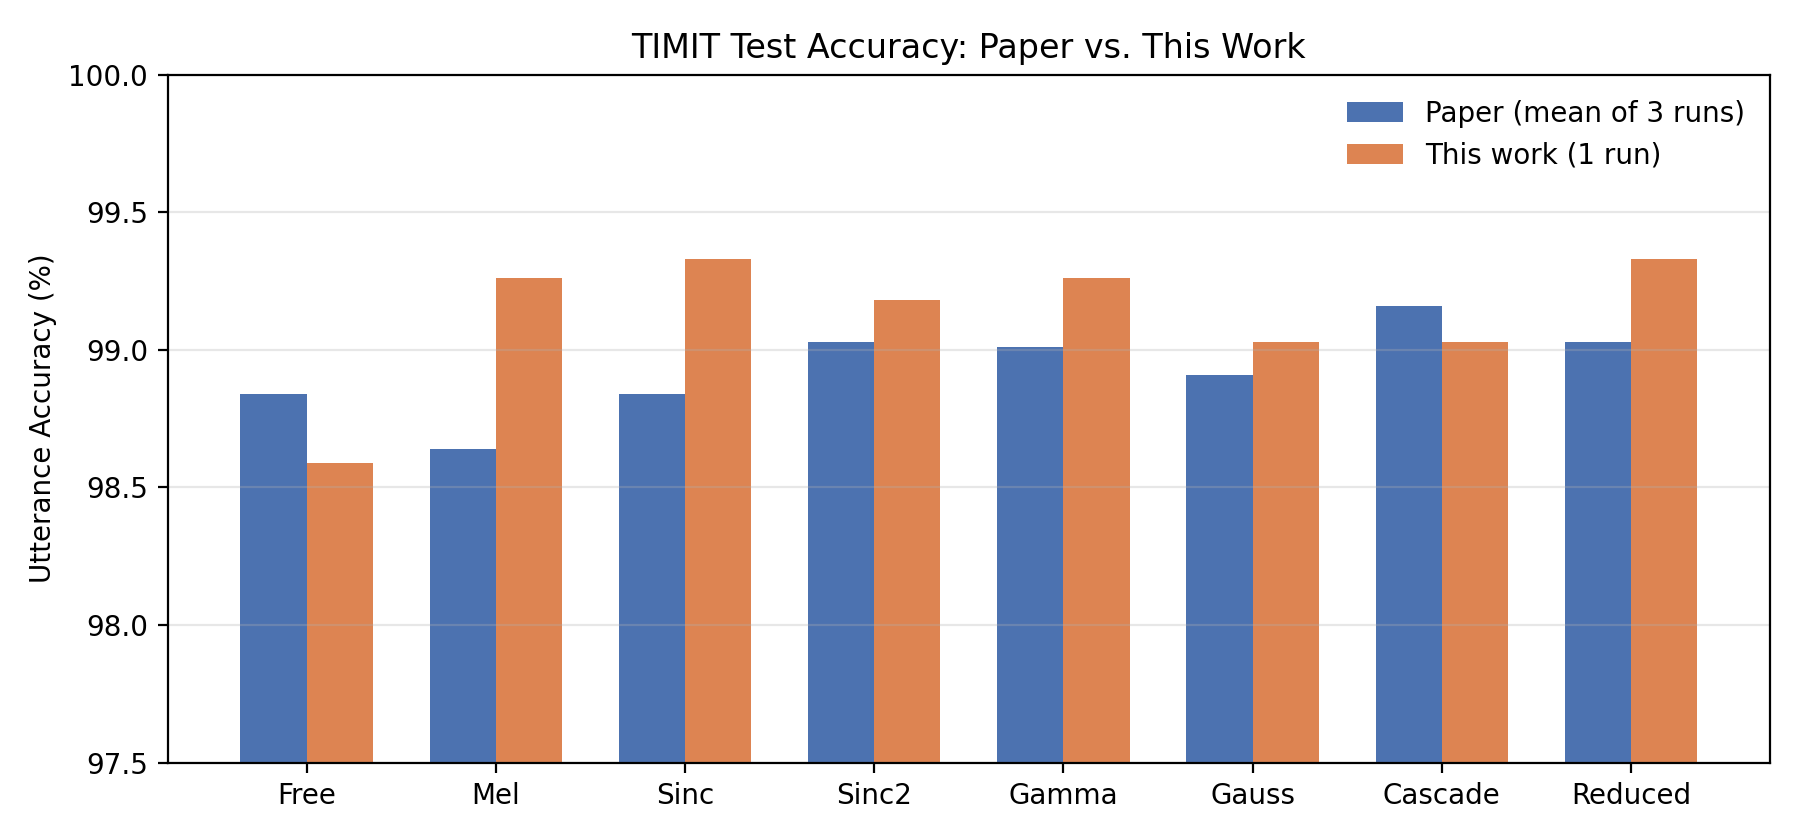
\includegraphics[width=0.92\textwidth]{bar_timit_acc.png}
\caption{TIMIT utterance accuracy: paper mean vs.\ this work.}
\label{fig:bar-timit}
\end{figure}

\subsection{LibriSpeech after fine-tuning}
\label{sec:libri}

After TIMIT pretraining, each model (except Mel) is fine-tuned for 20 epochs on LibriSpeech \texttt{dev-clean}. Table~\ref{tab:libri} reports (i)~best validation accuracy during fine-tuning and (ii)~utterance Acc / CER / FER on the held-out LibriSpeech \texttt{test-clean} set (2{,}620 utterances). The paper does not publish a LibriSpeech test table; these numbers document the intermediate adaptation stage before RAVDESS / VoxCeleb evaluation.

\paragraph{Evaluation protocol.}
Fine-tune validation follows the training split used in this project (speaker-held-out subset of \texttt{dev-clean}, plus 200 \texttt{test-clean} utterances for monitoring). Final LibriSpeech metrics use the full \texttt{test-clean} partition with evenly spaced chunks (at most 40 per utterance) and majority vote, which yields utterance CER/Acc comparable to the paper protocol while remaining computationally tractable.

\begin{table}[H]
\centering
\caption{LibriSpeech results after fine-tuning. Val = best utterance accuracy on the fine-tune validation split; Test = \texttt{test-clean}.}
\label{tab:libri}
\begin{tabular}{@{}lrrrrr@{}}
\toprule
\textbf{Method} & \textbf{FT train Acc} & \textbf{FT val Acc} & \textbf{Test Acc} & \textbf{Test CER} & \textbf{Test FER} \\
\midrule
Free-CNN & 96.89 & 89.33 & 94.47 & 5.53 & 13.88 \\
Sinc     & 97.88 & \textbf{90.25} & 88.44 & 11.56 & 19.95 \\
Sinc2    & \textbf{98.04} & 89.46 & \textbf{96.76} & \textbf{3.24} & 14.76 \\
Gamma    & 97.90 & 89.59 & 95.11 & 4.89 & 14.72 \\
Gauss    & 97.68 & 89.59 & 89.05 & 10.95 & 18.47 \\
Cascade  & 97.84 & 89.72 & 90.65 & 9.35 & 17.22 \\
Reduced  & 96.12 & 89.06 & 90.99 & 9.01 & 19.36 \\
\bottomrule
\end{tabular}
\end{table}

\begin{figure}[H]
\centering
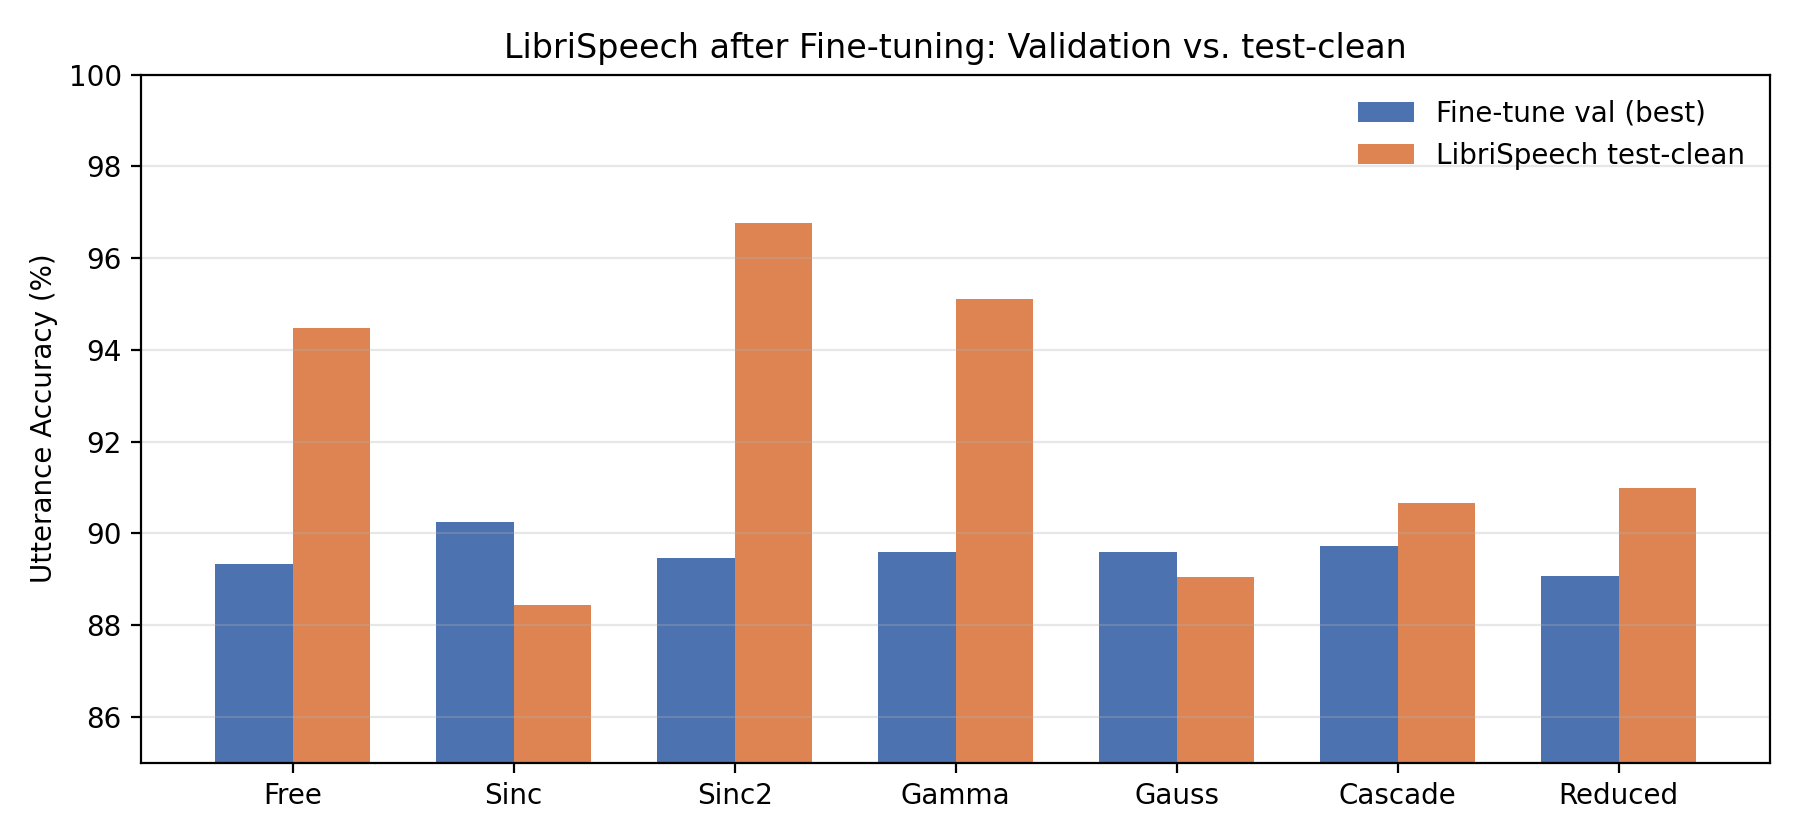
\includegraphics[width=0.92\textwidth]{bar_librispeech_acc.png}
\caption{LibriSpeech after fine-tuning: validation vs.\ \texttt{test-clean} accuracy.}
\label{fig:bar-libri}
\end{figure}

Sinc2 attains the strongest \texttt{test-clean} accuracy (96.76\%). Fine-tune validation accuracies lie near $89$--$90\%$ for all frontends; the gap between validation and \texttt{test-clean} for some models (e.g., Sinc) reflects the smaller, partially mixed validation monitor used during training rather than a pure \texttt{test-clean} hold-out.

\subsection{RAVDESS (out-of-domain)}
\label{sec:ravdess}

Table~\ref{tab:ravdess} reports RAVDESS accuracy after LibriSpeech fine-tuning (paper Table~8). Cascade remains our strongest model (95.21\%), 2.78\,pp below the paper's Cascade (97.99\%). Sinc2 nearly matches the paper ($-0.28$\,pp); Gauss slightly exceeds it ($+0.28$\,pp). Free-CNN exhibits the largest deficit ($-9.86$\,pp), consistent with weaker inductive bias under limited fine-tuning.

\begin{table}[H]
\centering
\caption{RAVDESS accuracy after fine-tuning (\%).}
\label{tab:ravdess}
\begin{tabular}{@{}lrrr@{}}
\toprule
\textbf{Method} & \textbf{Paper} & \textbf{Ours} & $\boldsymbol{\Delta}$ \\
\midrule
Free-CNN & 93.54 & 83.68 & $-9.86$ \\
Sinc     & 96.32 & 93.33 & $-2.99$ \\
Sinc2    & 94.86 & 94.58 & $-0.28$ \\
Gamma    & 97.78 & 92.71 & $-5.07$ \\
Gauss    & 93.19 & \textbf{93.47} & $\boldsymbol{+0.28}$ \\
Cascade  & \textbf{97.99} & 95.21 & $-2.78$ \\
Reduced  & 96.11 & 90.83 & $-5.28$ \\
\bottomrule
\end{tabular}
\end{table}

\begin{figure}[H]
\centering
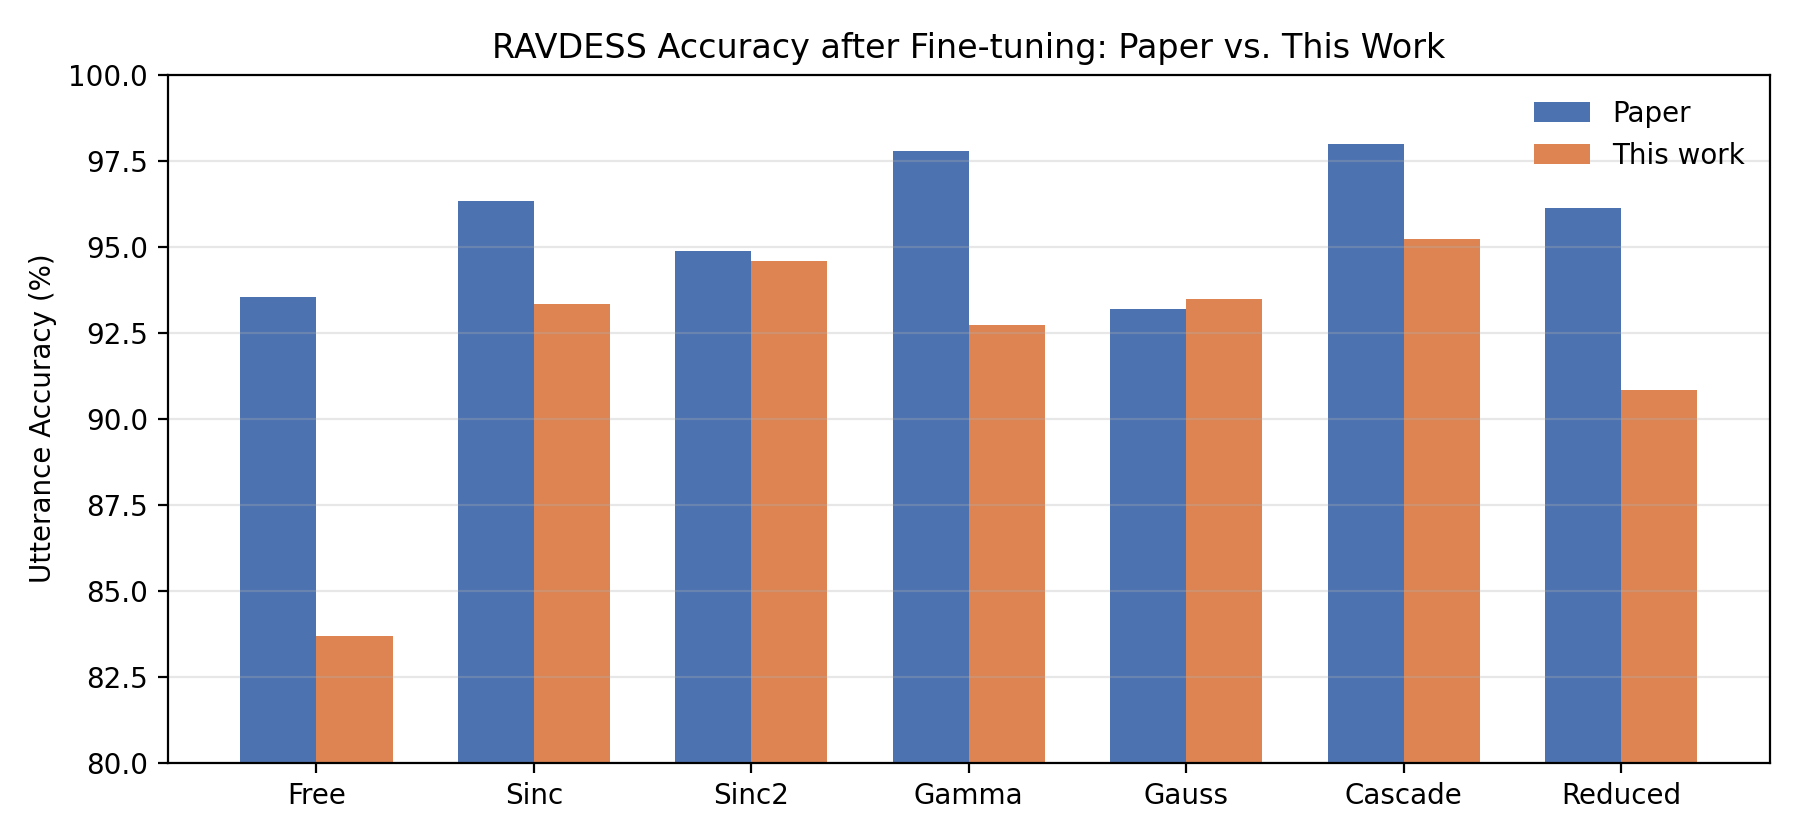
\includegraphics[width=0.92\textwidth]{bar_ravdess_acc.png}
\caption{RAVDESS accuracy after fine-tuning: paper vs.\ this work.}
\label{fig:bar-rav}
\end{figure}

\subsection{VoxCeleb1-test (out-of-domain)}
\label{sec:vox}

Table~\ref{tab:vox} compares VoxCeleb results (paper Table~7 reports full VoxCeleb1; we evaluate VoxCeleb1-test only). Reduced (95.28\%) and Sinc2 (95.12\%) are closest to the paper (gaps of $2.16$ and $1.21$\,pp). Free-CNN again shows the largest shortfall.

\begin{table}[H]
\centering
\caption{VoxCeleb accuracy after fine-tuning (\%). Paper: full set; ours: test partition.}
\label{tab:vox}
\begin{tabular}{@{}lrrr@{}}
\toprule
\textbf{Method} & \textbf{Paper} & \textbf{Ours} & $\boldsymbol{\Delta}$ \\
\midrule
Free-CNN & 97.48 & 88.51 & $-8.97$ \\
Sinc     & \textbf{97.66} & 91.24 & $-6.42$ \\
Sinc2    & 96.33 & 95.12 & $-1.21$ \\
Gamma    & 97.17 & 93.39 & $-3.78$ \\
Gauss    & 96.74 & 89.74 & $-7.00$ \\
Cascade  & 97.27 & 91.01 & $-6.26$ \\
Reduced  & 97.44 & \textbf{95.28} & $-2.16$ \\
\bottomrule
\end{tabular}
\end{table}

\begin{figure}[H]
\centering
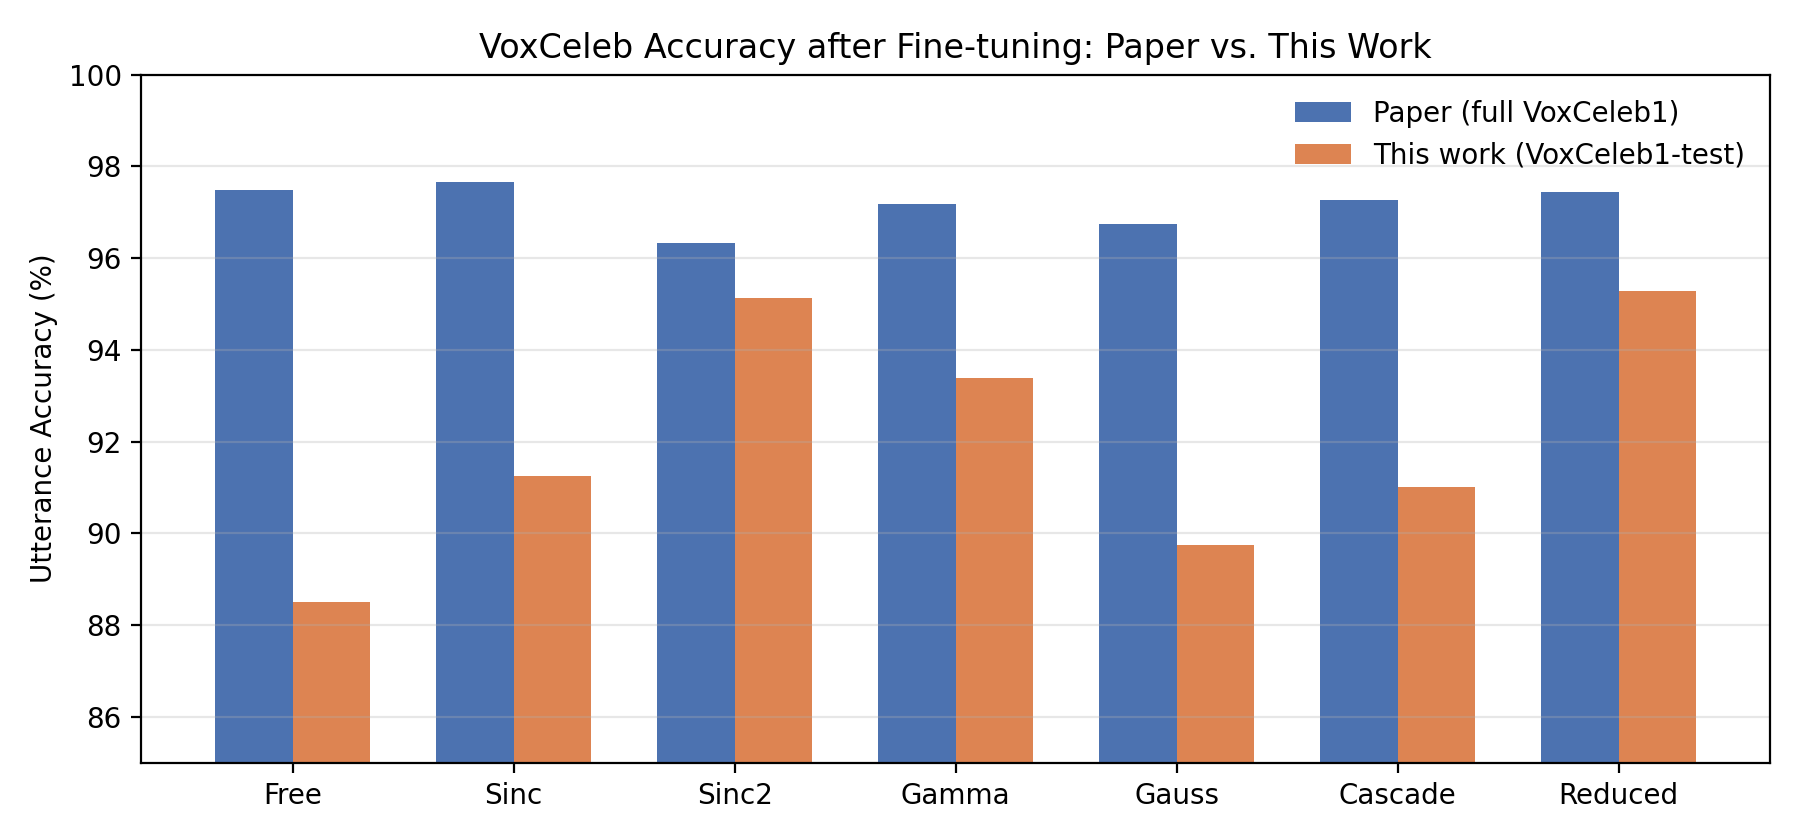
\includegraphics[width=0.92\textwidth]{bar_vox_acc.png}
\caption{VoxCeleb accuracy after fine-tuning: paper (full) vs.\ this work (test).}
\label{fig:bar-vox}
\end{figure}

% ============================================================
\section{Training Dynamics}
\label{sec:curves}
% ============================================================

Figures~\ref{fig:cascade-timit-curves}--\ref{fig:reduced-ft-curves} show loss and accuracy trajectories for Cascade and Reduced under TIMIT training and LibriSpeech fine-tuning. Both systems converge rapidly on TIMIT; validation accuracy plateaus near $99\%$ within the first few dozen epochs, supporting the adequacy of a 50-epoch budget for in-domain evaluation. Fine-tuning further reduces loss while improving RAVDESS/Vox generalization (Sec.~\ref{sec:ravdess}--\ref{sec:vox}).

\begin{figure}[H]
\centering
\begin{subfigure}[t]{0.48\textwidth}
  \centering
  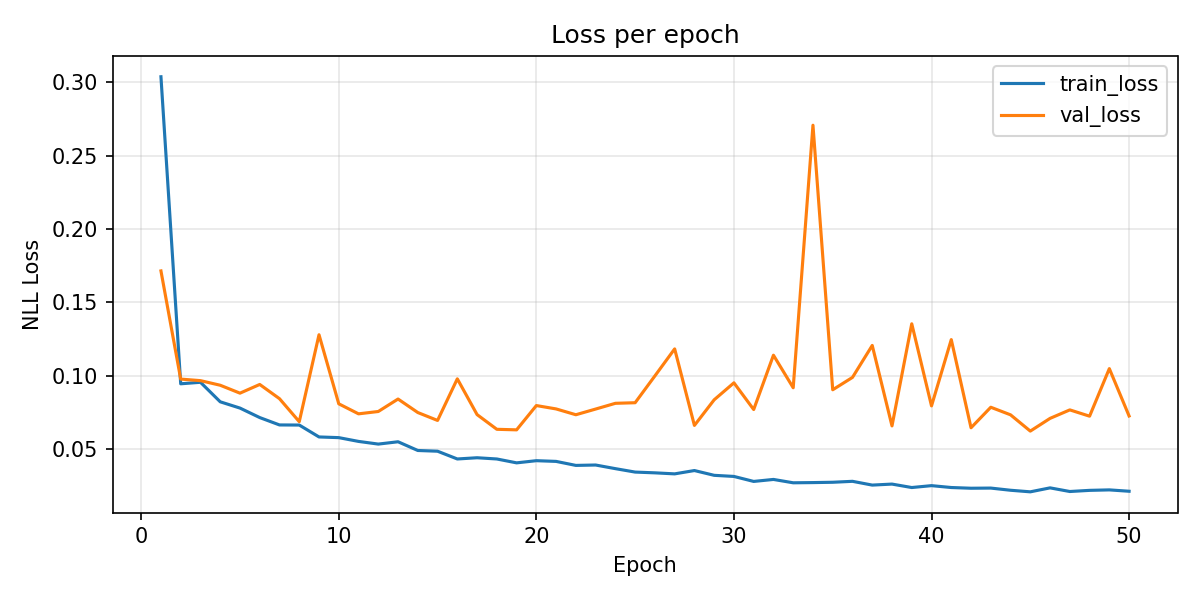
\includegraphics[width=\linewidth]{cascade_timit_loss.png}
  \caption{Loss}
\end{subfigure}\hfill
\begin{subfigure}[t]{0.48\textwidth}
  \centering
  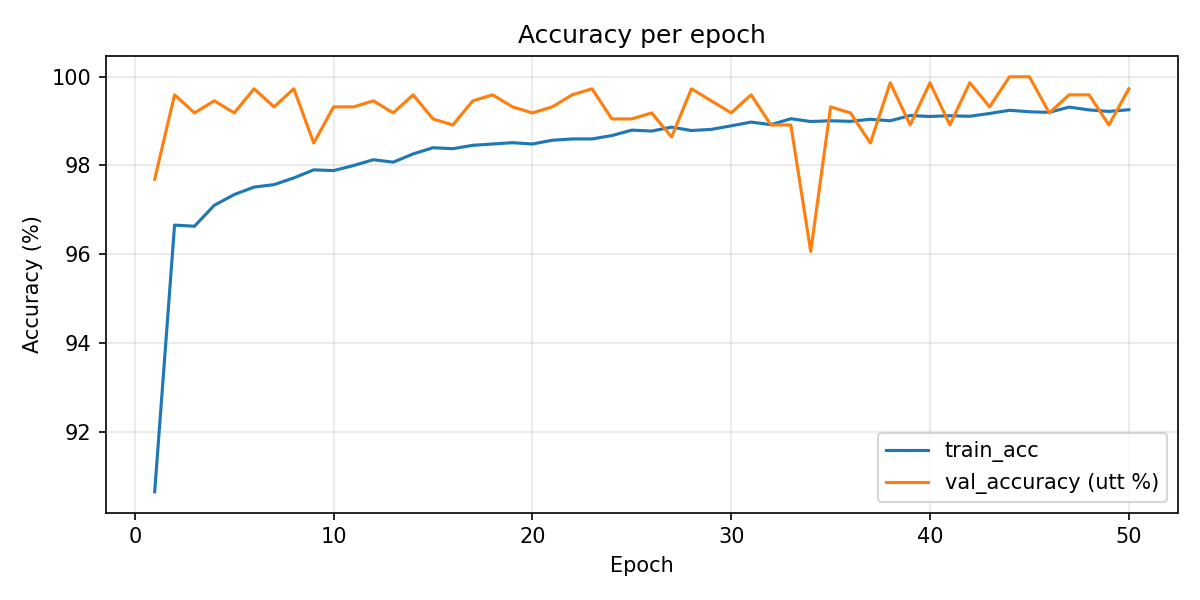
\includegraphics[width=\linewidth]{cascade_timit_acc.png}
  \caption{Accuracy}
\end{subfigure}
\caption{Cascade --- TIMIT training (50 epochs).}
\label{fig:cascade-timit-curves}
\end{figure}

\begin{figure}[H]
\centering
\begin{subfigure}[t]{0.48\textwidth}
  \centering
  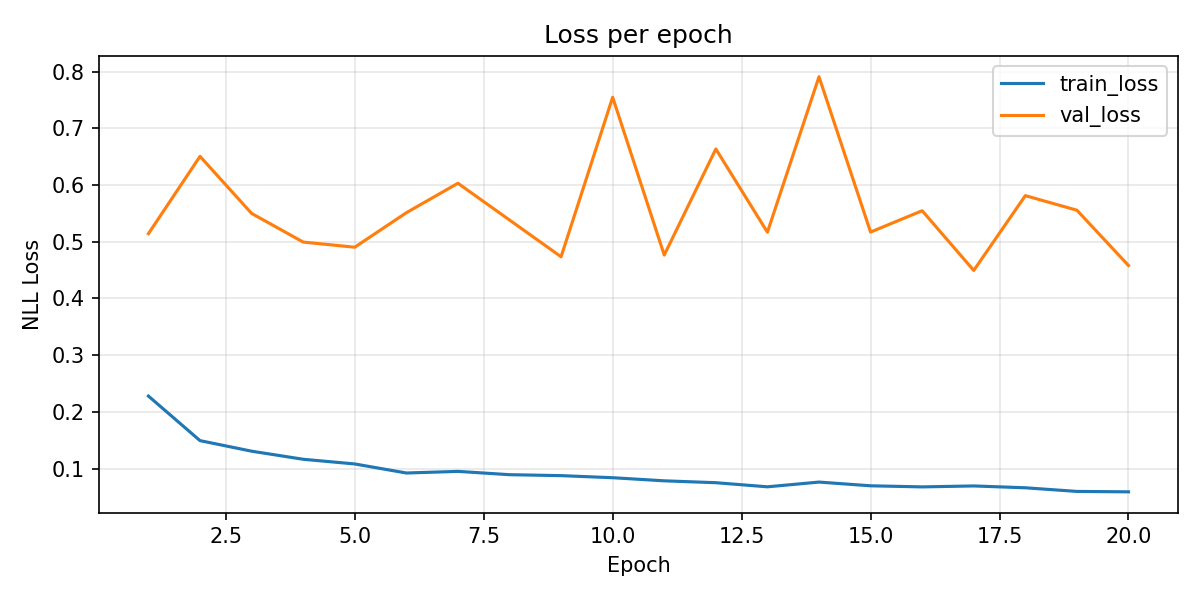
\includegraphics[width=\linewidth]{cascade_ft_loss.png}
  \caption{Loss}
\end{subfigure}\hfill
\begin{subfigure}[t]{0.48\textwidth}
  \centering
  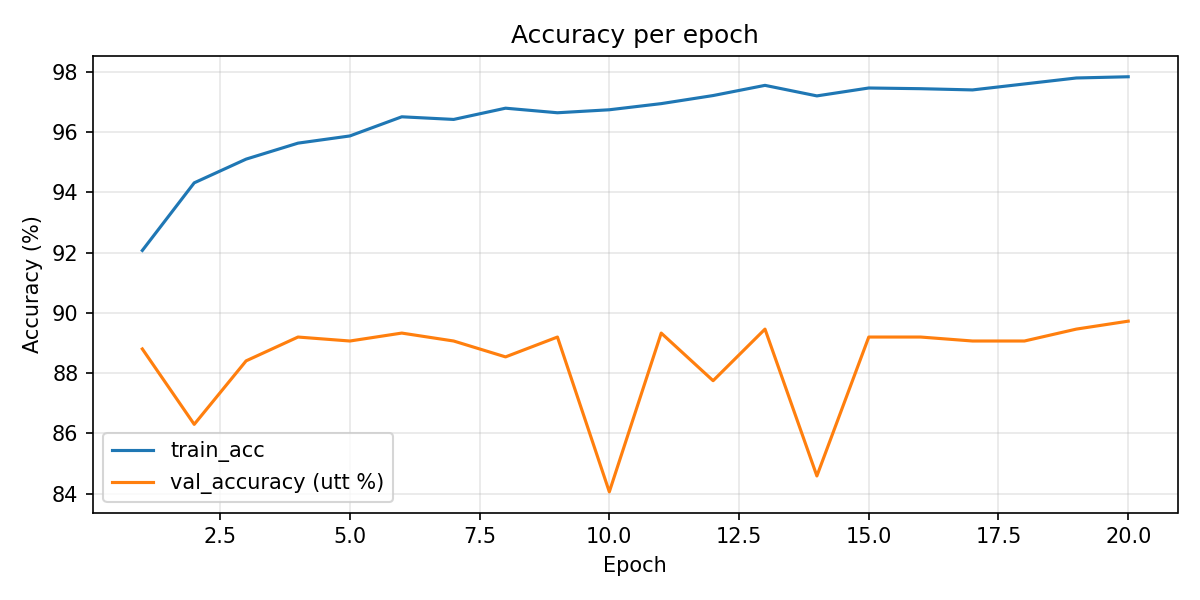
\includegraphics[width=\linewidth]{cascade_ft_acc.png}
  \caption{Accuracy}
\end{subfigure}
\caption{Cascade --- LibriSpeech fine-tuning (20 epochs).}
\label{fig:cascade-ft-curves}
\end{figure}

\begin{figure}[H]
\centering
\begin{subfigure}[t]{0.48\textwidth}
  \centering
  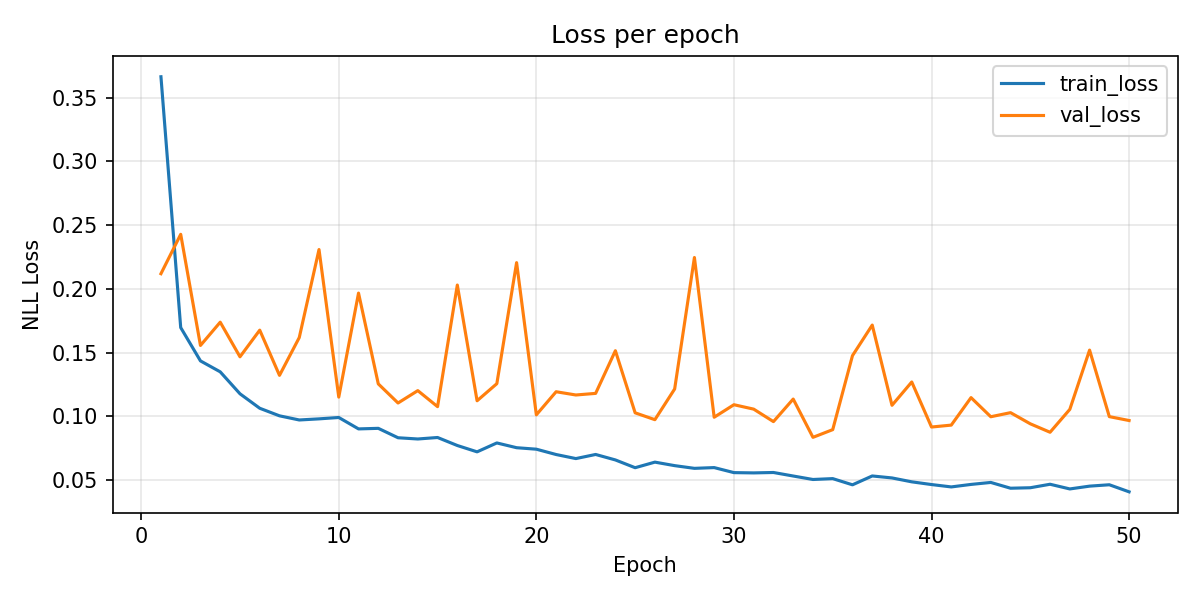
\includegraphics[width=\linewidth]{reduced_timit_loss.png}
  \caption{Loss}
\end{subfigure}\hfill
\begin{subfigure}[t]{0.48\textwidth}
  \centering
  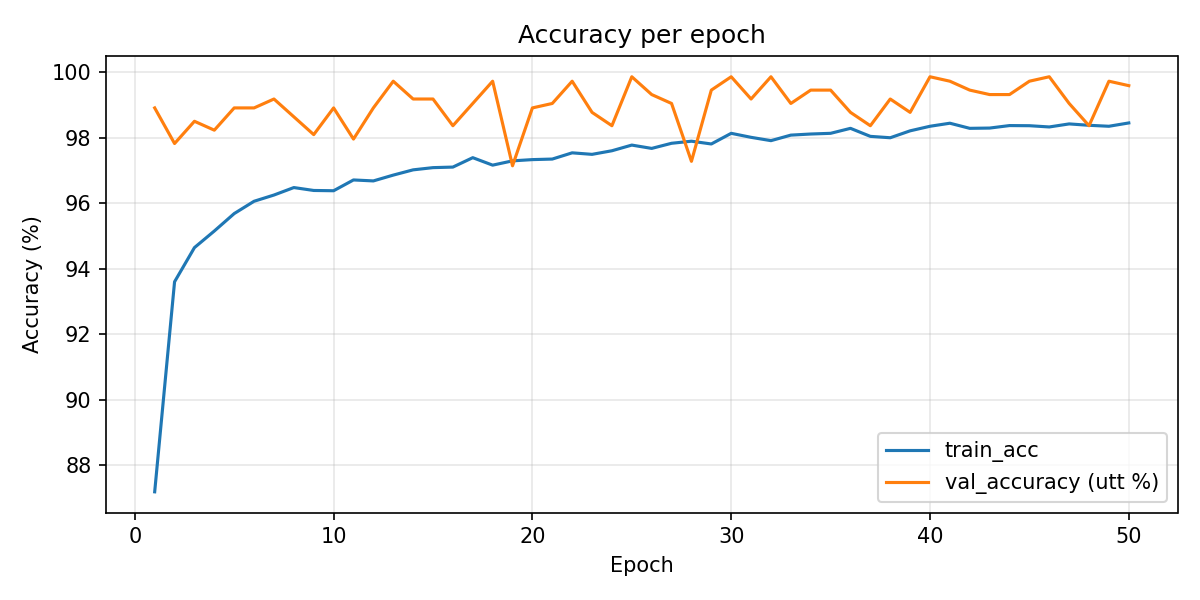
\includegraphics[width=\linewidth]{reduced_timit_acc.png}
  \caption{Accuracy}
\end{subfigure}
\caption{Reduced --- TIMIT retraining after pole pruning (50 epochs).}
\label{fig:reduced-timit-curves}
\end{figure}

\begin{figure}[H]
\centering
\begin{subfigure}[t]{0.48\textwidth}
  \centering
  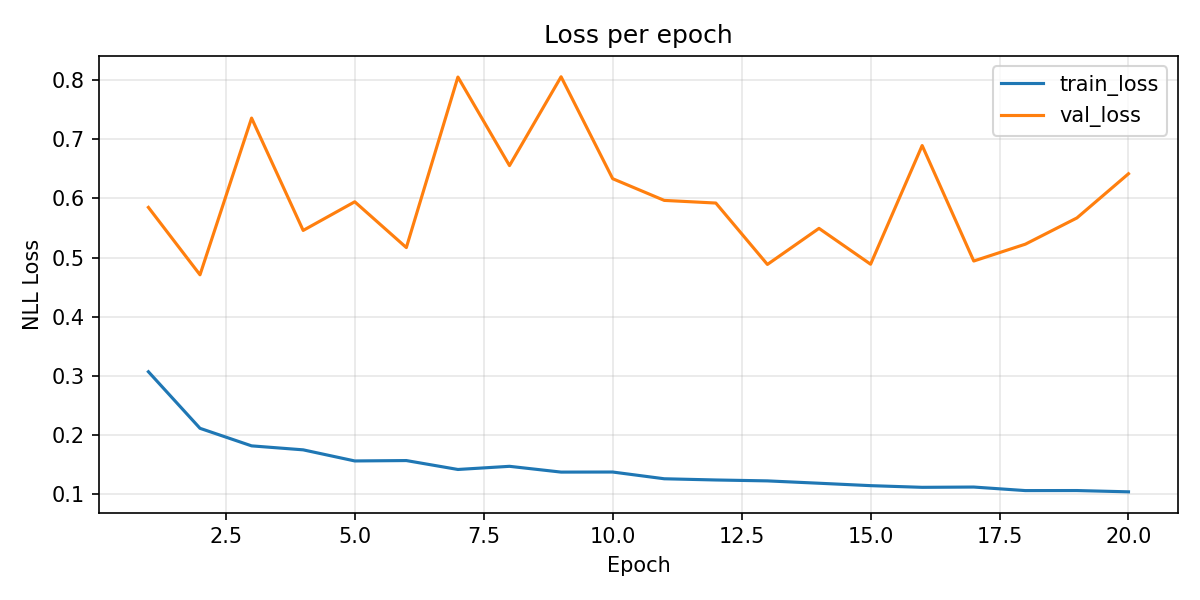
\includegraphics[width=\linewidth]{reduced_ft_loss.png}
  \caption{Loss}
\end{subfigure}\hfill
\begin{subfigure}[t]{0.48\textwidth}
  \centering
  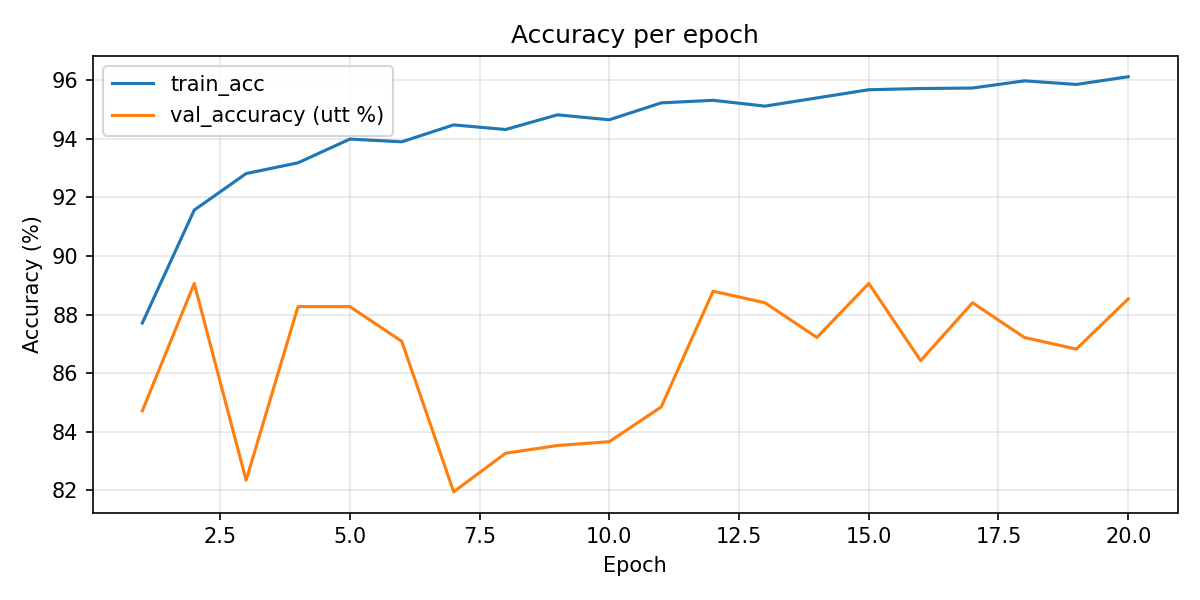
\includegraphics[width=\linewidth]{reduced_ft_acc.png}
  \caption{Accuracy}
\end{subfigure}
\caption{Reduced --- LibriSpeech fine-tuning (20 epochs).}
\label{fig:reduced-ft-curves}
\end{figure}

% ============================================================
\section{Pole Reduction on the Complex Plane}
\label{sec:poles}
% ============================================================

Figure~\ref{fig:poles} visualizes Cascade poles before and after mean-shift clustering. Left: all Cascade poles (two per filter, upper half-plane), lying inside the unit circle as required for stable band-pass responses. Right: retained cluster centroids after mean-shift and Nyquist filtering, which become the frozen Reduced bank ($N{=}26$). The reduction concentrates filters where Cascade poles are densest, typically in perceptually relevant mid-frequency regions, while discarding redundant near-duplicate poles.

\begin{figure}[H]
\centering
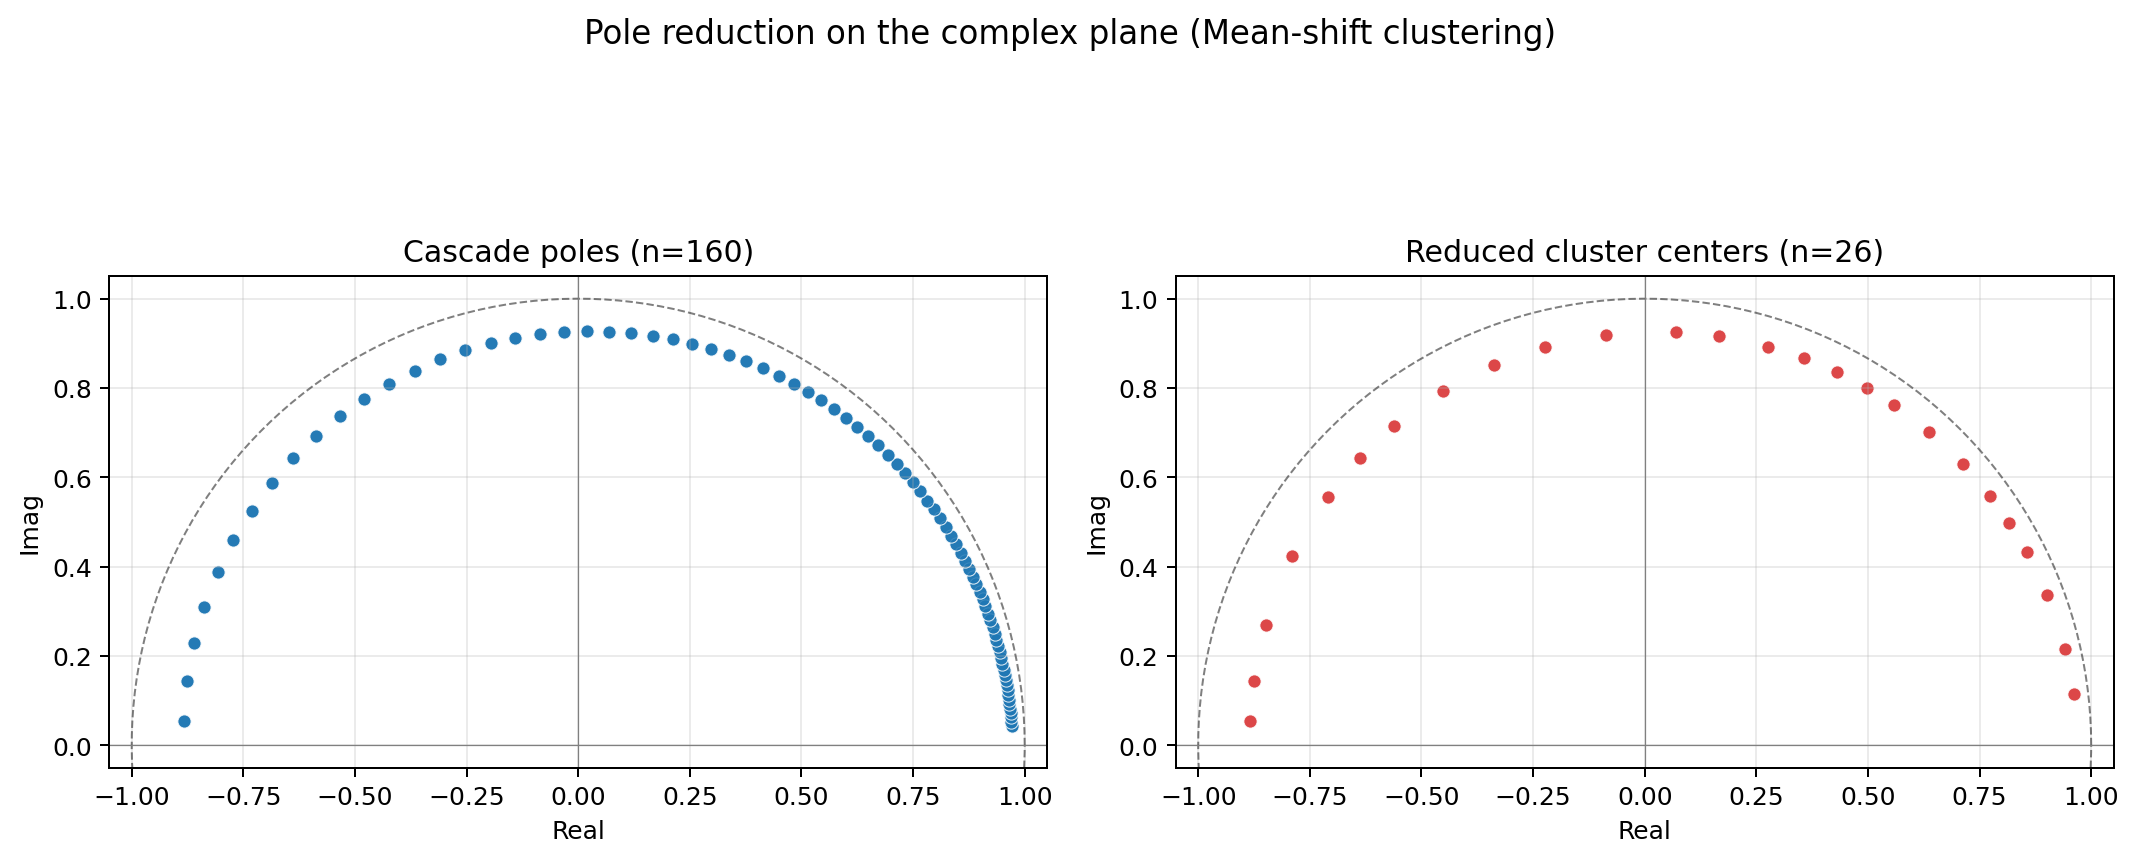
\includegraphics[width=0.98\textwidth]{pole_reduction.png}
\caption{Pole reduction on the complex plane. Left: Cascade poles. Right: mean-shift cluster centers used by the Reduced frontend.}
\label{fig:poles}
\end{figure}

% ============================================================
\section{Filter Interpretability Analysis}
\label{sec:analysis}
% ============================================================

\subsection{Cascade}

Figure~\ref{fig:cascade-analysis} shows the accumulative magnitude response and center-frequency histogram of the trained Cascade bank; Figure~\ref{fig:cascade-tsne-qf} shows t-SNE of convolutional features and the quality-factor trajectory $Q(f_c)$. Male and female clusters are well separated in the embedding space, consistent with the high TIMIT accuracy in Table~\ref{tab:timit}.

\begin{figure}[H]
\centering
\begin{subfigure}[t]{0.48\textwidth}
  \centering
  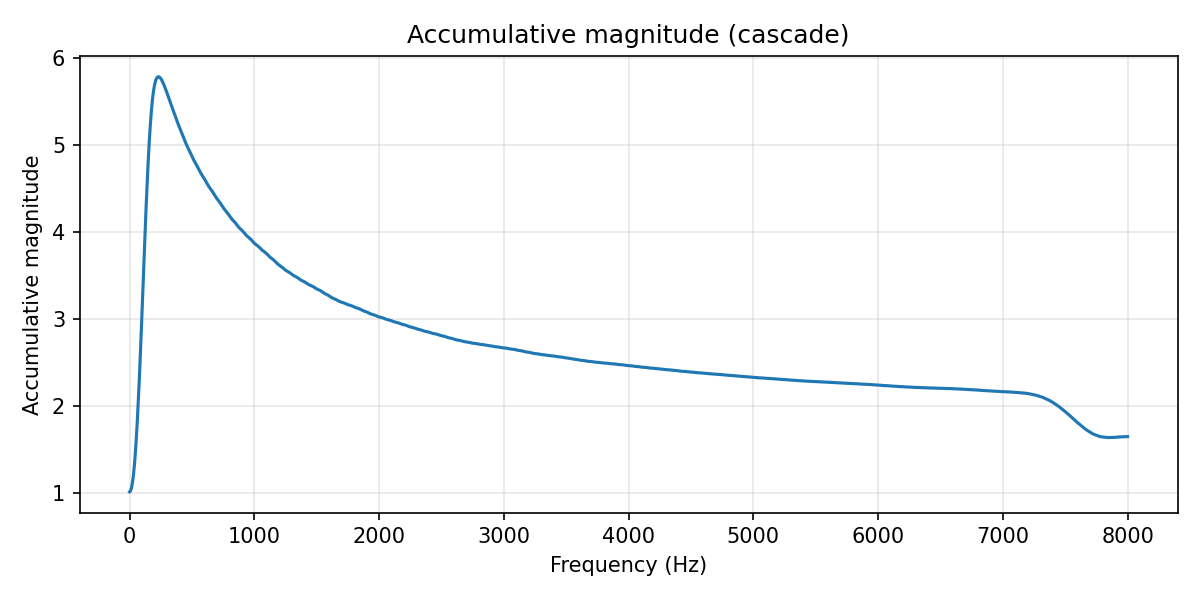
\includegraphics[width=\linewidth]{cascade_accum_mag.png}
  \caption{Accumulative magnitude}
\end{subfigure}\hfill
\begin{subfigure}[t]{0.48\textwidth}
  \centering
  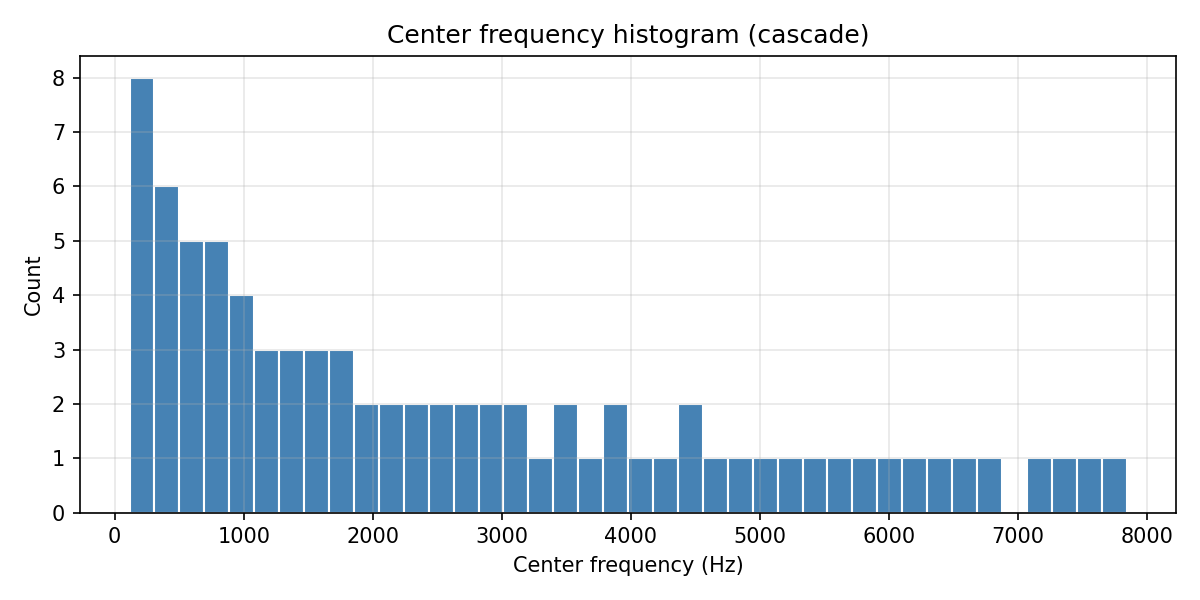
\includegraphics[width=\linewidth]{cascade_fc_hist.png}
  \caption{Center-frequency histogram}
\end{subfigure}
\caption{Cascade filter-bank analysis after TIMIT training.}
\label{fig:cascade-analysis}
\end{figure}

\begin{figure}[H]
\centering
\begin{subfigure}[t]{0.48\textwidth}
  \centering
  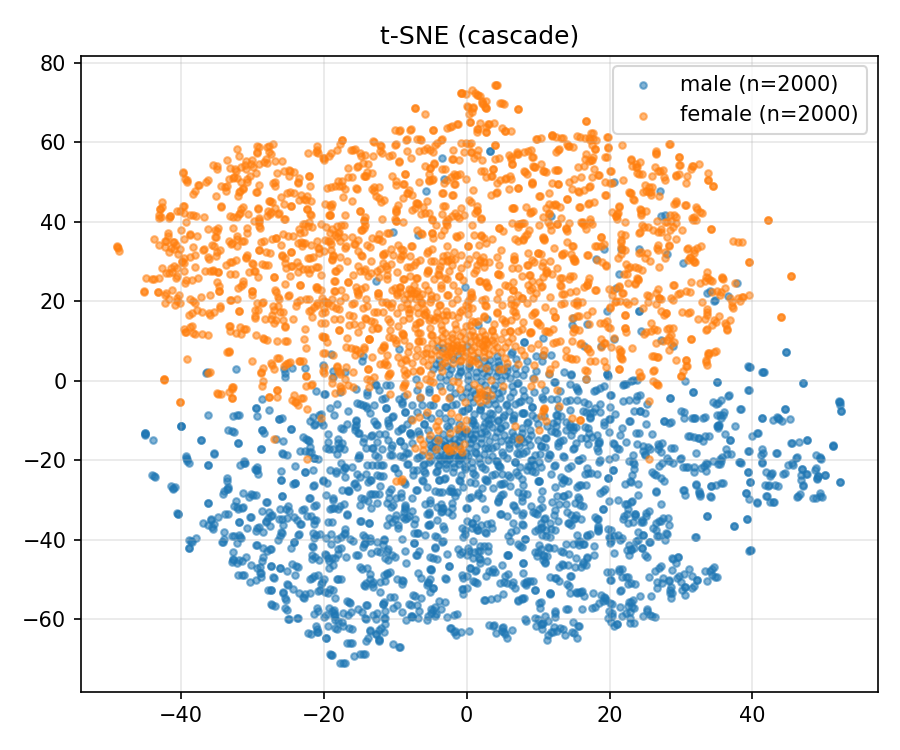
\includegraphics[width=\linewidth]{cascade_tsne.png}
  \caption{t-SNE of Conv features}
\end{subfigure}\hfill
\begin{subfigure}[t]{0.48\textwidth}
  \centering
  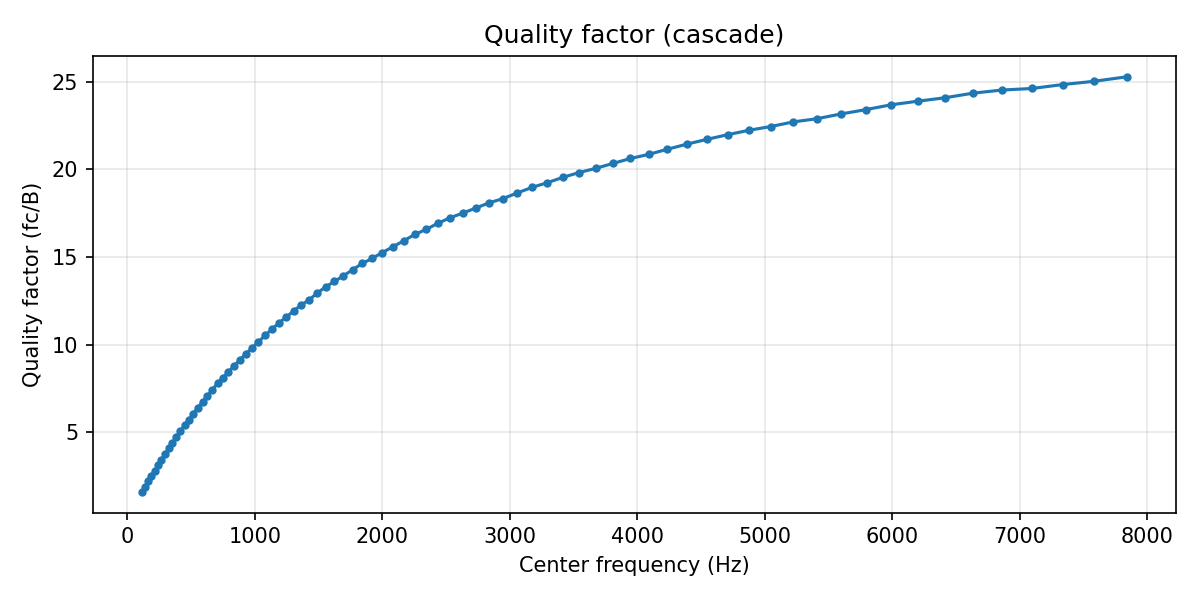
\includegraphics[width=\linewidth]{cascade_qf.png}
  \caption{Quality factor $Q{=}f_c/B$}
\end{subfigure}
\caption{Cascade: feature separability and quality-factor profile.}
\label{fig:cascade-tsne-qf}
\end{figure}

\subsection{Reduced (overview)}

The Reduced frontend is the paper's compact architecture obtained by pruning Cascade poles. A dedicated case study with all metrics and figures is given in Sec.~\ref{sec:reduced-case}.

% ============================================================
\section{Case Study: The Reduced Model}
\label{sec:reduced-case}
% ============================================================

The Reduced model is the central practical contribution of~\cite{fayyazi2023}: a much smaller frozen filter bank that retains Cascade-level accuracy. This section consolidates its construction, hyperparameters, quantitative results on every evaluation set used in this project, training curves, pole-reduction geometry, and filter interpretability plots (TIMIT and post--fine-tune RAVDESS).

\subsection{Construction and configuration}

\begin{enumerate}[leftmargin=1.6em,itemsep=0.3em]
  \item Train Cascade on TIMIT (80 dual-Gaussian filters $\Rightarrow$ 160 poles).
  \item Map poles to the complex plane; cluster with Mean-Shift (target $\approx 40$).
  \item Realize cluster centers as triangular (Sinc2-style) FIR filters of length 257.
  \item Freeze Conv1; retrain Conv2/Conv3/FC on TIMIT for 50 epochs.
  \item Fine-tune on LibriSpeech \texttt{dev-clean} for 20 epochs; evaluate on \texttt{test-clean}, RAVDESS, and VoxCeleb1-test.
\end{enumerate}

In our run, Mean-Shift retained \textbf{26} filters (paper target $\approx 40$; see Sec.~\ref{sec:poles}). Conv1 is frozen thereafter. Optimizer, learning rate, and batch size match the other frontends (RMSprop, $10^{-3}$, 128).

\subsection{Summary of results (Reduced only)}

Table~\ref{tab:reduced-summary} collects every reported metric for Reduced. Where the paper publishes a number, we include it for comparison.

\begin{table}[H]
\centering
\caption{Reduced model --- complete metrics. Paper LibriSpeech test is not published.}
\label{tab:reduced-summary}
\small
\begin{tabular}{@{}llrrr@{}}
\toprule
\textbf{Set} & \textbf{Source} & \textbf{Acc (\%)} & \textbf{CER (\%)} & \textbf{FER (\%)} \\
\midrule
TIMIT test
  & Paper (Table~4 / Sec.~4.3)
  & 99.03 & 0.97 & 3.94 \\
TIMIT test
  & Ours
  & \textbf{99.33} & \textbf{0.67} & 3.81 \\
\midrule
LibriSpeech FT val (best)
  & Ours
  & 89.06 & --- & --- \\
LibriSpeech \texttt{test-clean}
  & Ours
  & 90.99 & 9.01 & 19.36 \\
\midrule
RAVDESS (after FT)
  & Paper (Table~8)
  & 96.11 & --- & --- \\
RAVDESS (after FT)
  & Ours
  & 90.83 & 9.17 & 19.83 \\
\midrule
VoxCeleb (after FT)
  & Paper (Table~7, full set)
  & 97.44 & --- & --- \\
VoxCeleb1-test (after FT)
  & Ours
  & 95.28 & 4.72 & 17.78 \\
\bottomrule
\end{tabular}
\end{table}

\begin{figure}[H]
\centering
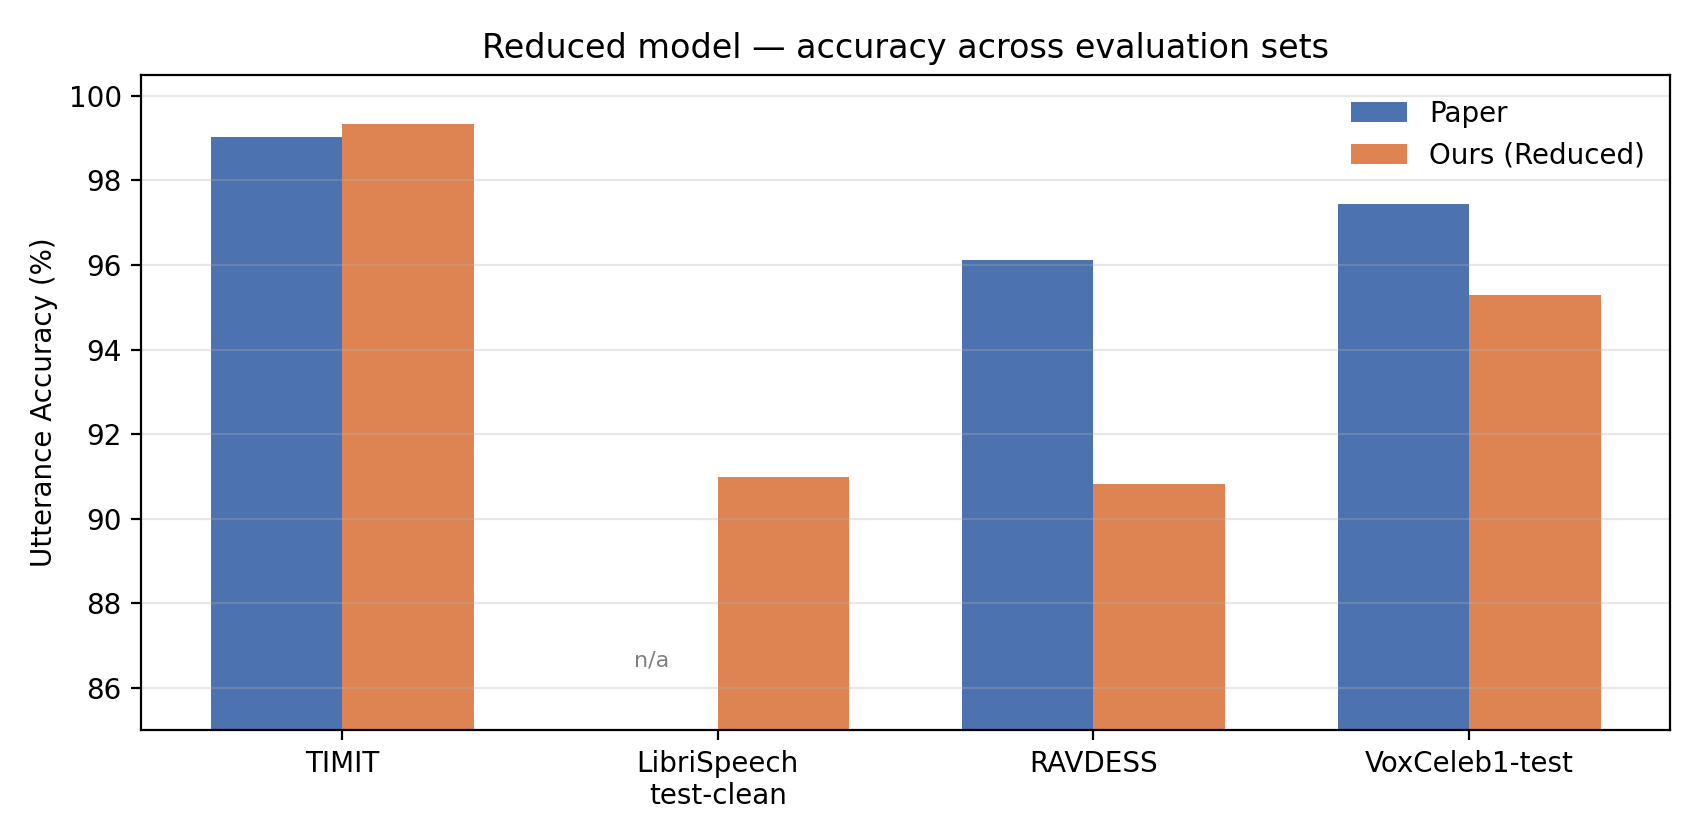
\includegraphics[width=0.92\textwidth]{bar_reduced_all_sets.png}
\caption{Reduced accuracy across evaluation sets (paper vs.\ this work). Paper does not report LibriSpeech test accuracy.}
\label{fig:bar-reduced-all}
\end{figure}

\paragraph{Takeaways.}
On TIMIT, Reduced is our best CER ($0.67\%$), slightly above the paper mean. On VoxCeleb1-test it is our best OOD model among all frontends ($95.28\%$, $-2.16$\,pp vs.\ paper full-set). The RAVDESS gap ($-5.28$\,pp) is consistent with the shorter fine-tuning budget.

\subsection{Pole reduction (Cascade $\to$ Reduced)}

Figure~\ref{fig:poles-reduced-case} repeats the complex-plane view: 160 Cascade poles collapse to 26 mean-shift centers that define the frozen Reduced bank. Poles lie on a thin arc inside the unit circle (similar bandwidths); angular density is highest at low frequencies.

\begin{figure}[H]
\centering
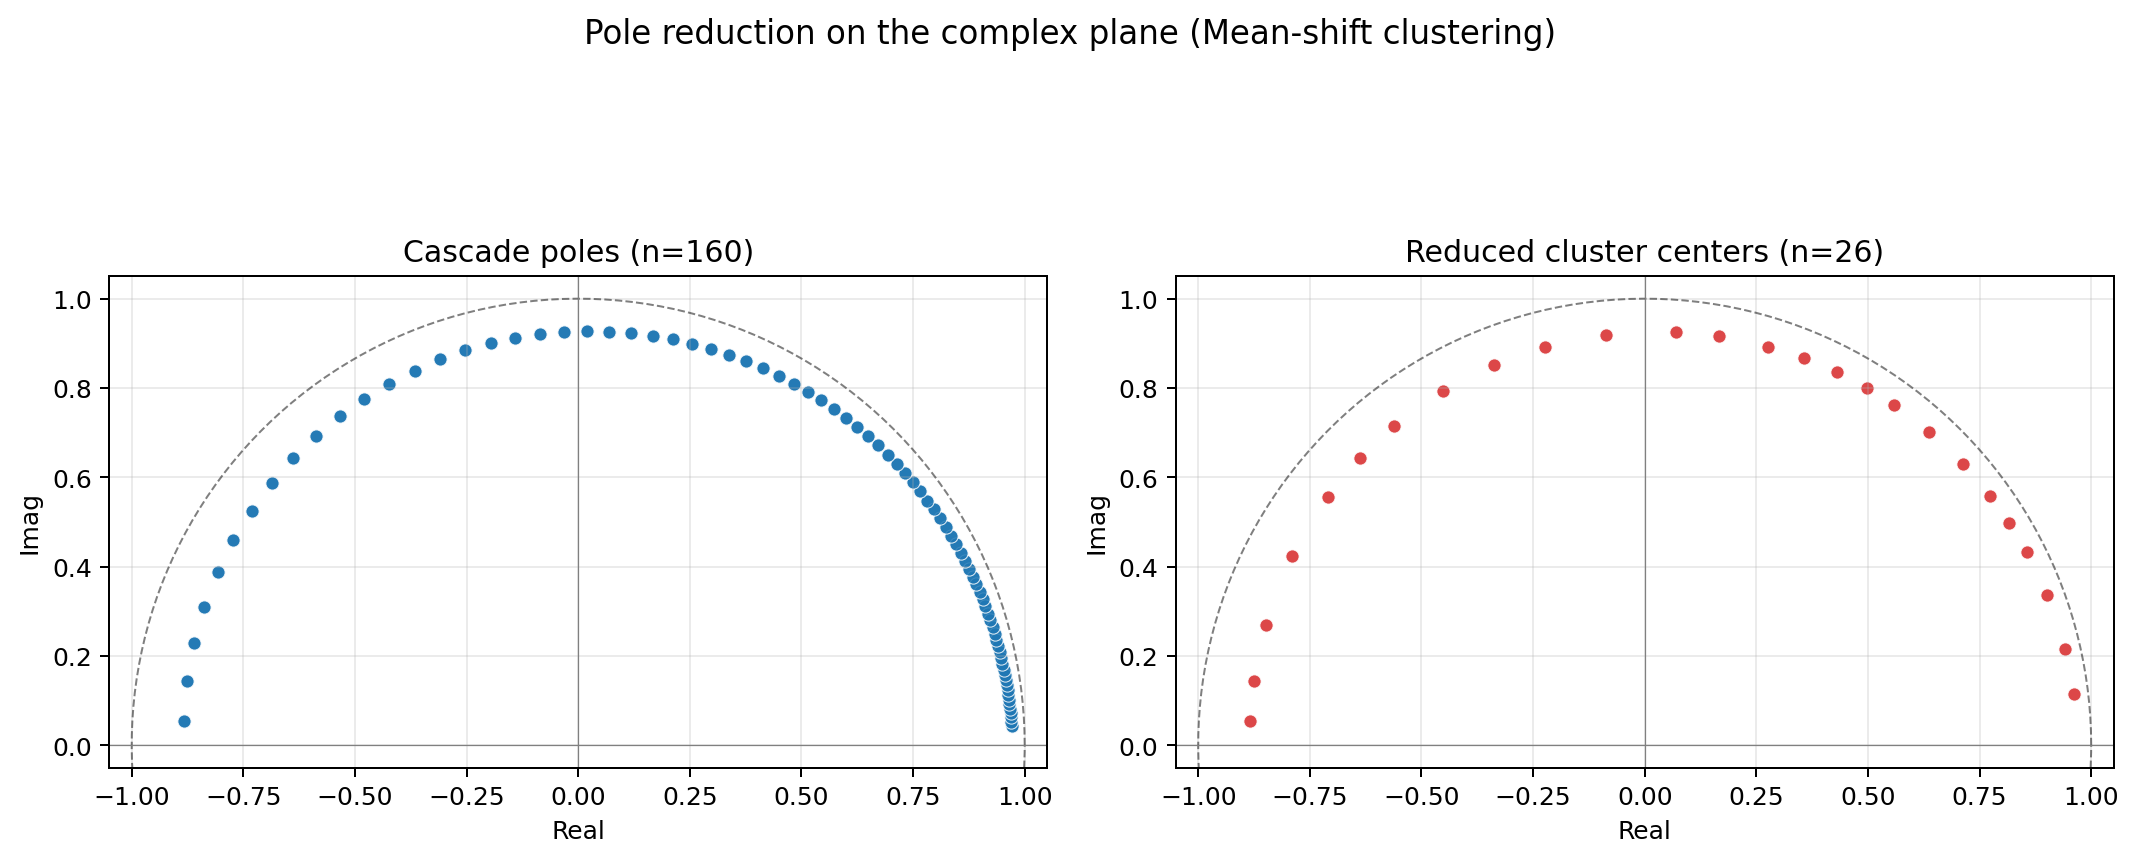
\includegraphics[width=0.98\textwidth]{pole_reduction.png}
\caption{Reduced construction: Cascade poles (left) and retained mean-shift centers (right, $N{=}26$).}
\label{fig:poles-reduced-case}
\end{figure}

\subsection{Training dynamics}

Figures~\ref{fig:reduced-timit-curves} and~\ref{fig:reduced-ft-curves} (also shown in Sec.~\ref{sec:curves}) document TIMIT retraining and LibriSpeech fine-tuning. Validation accuracy on TIMIT exceeds $99\%$ early; fine-tuning validation settles near $89\%$.

\begin{figure}[H]
\centering
\begin{subfigure}[t]{0.48\textwidth}
  \centering
  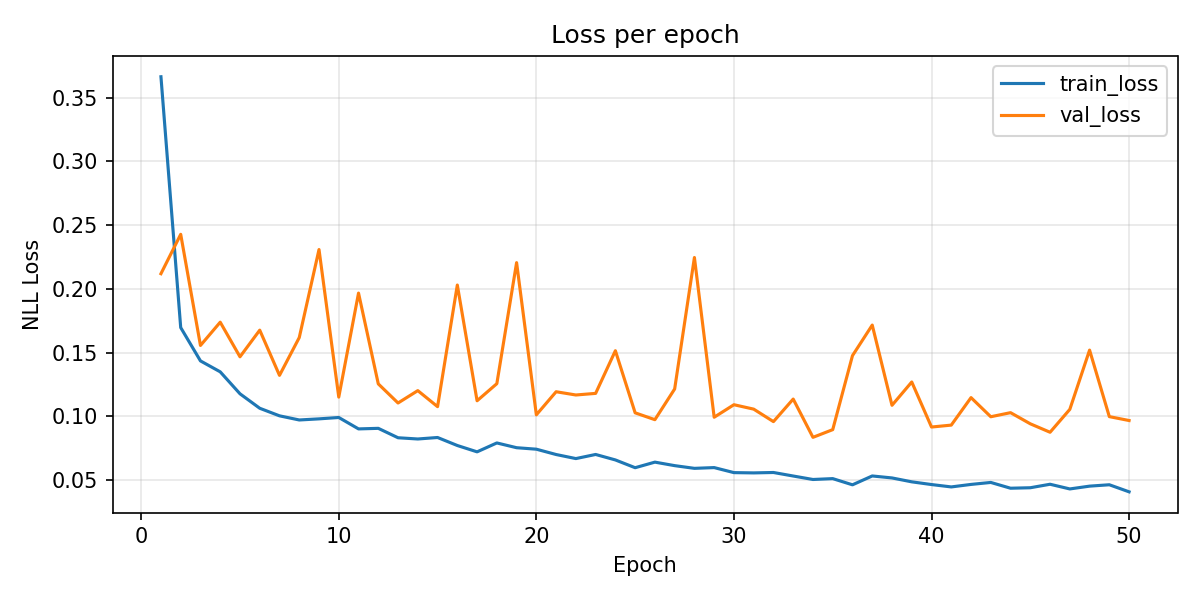
\includegraphics[width=\linewidth]{reduced_timit_loss.png}
  \caption{Loss}
\end{subfigure}\hfill
\begin{subfigure}[t]{0.48\textwidth}
  \centering
  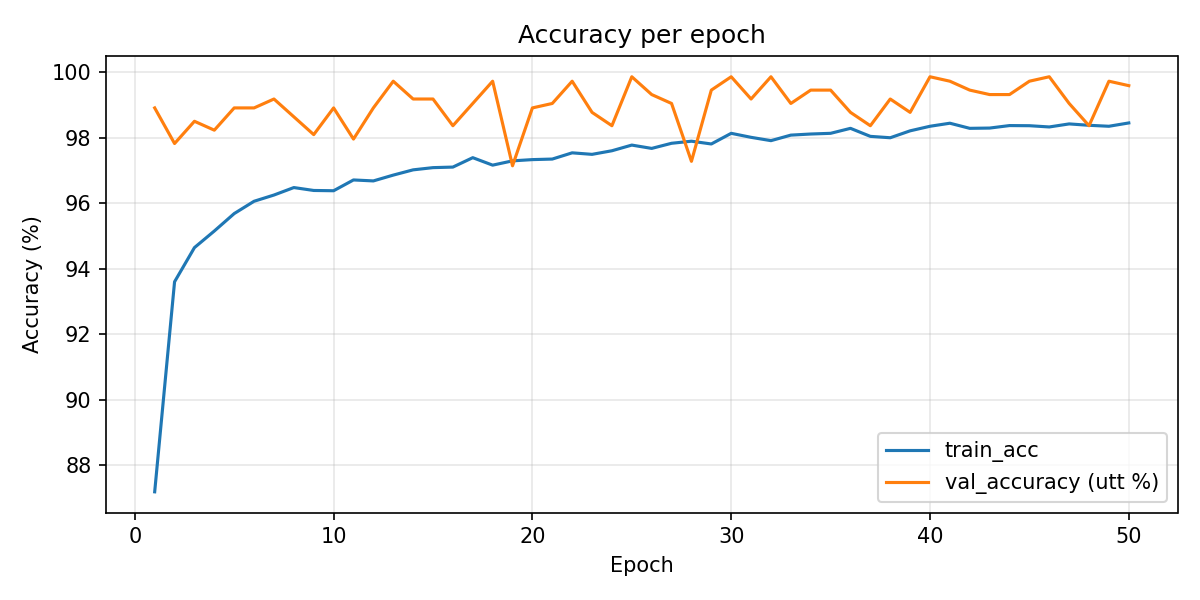
\includegraphics[width=\linewidth]{reduced_timit_acc.png}
  \caption{Accuracy}
\end{subfigure}
\caption{Reduced --- TIMIT retraining (50 epochs, frozen Conv1).}
\end{figure}

\begin{figure}[H]
\centering
\begin{subfigure}[t]{0.48\textwidth}
  \centering
  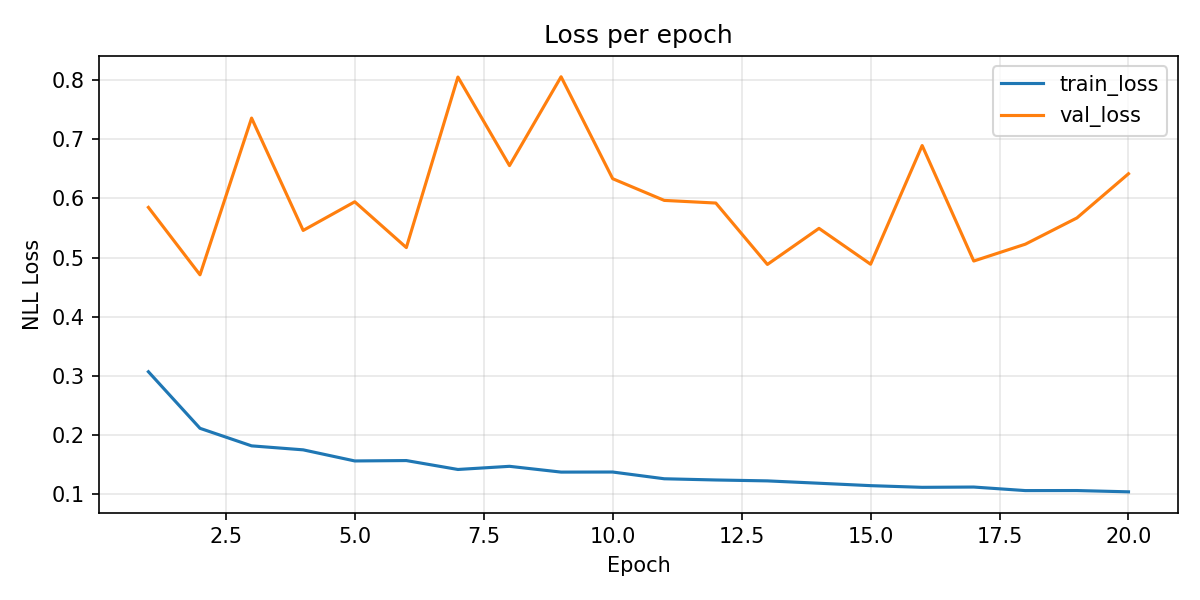
\includegraphics[width=\linewidth]{reduced_ft_loss.png}
  \caption{Loss}
\end{subfigure}\hfill
\begin{subfigure}[t]{0.48\textwidth}
  \centering
  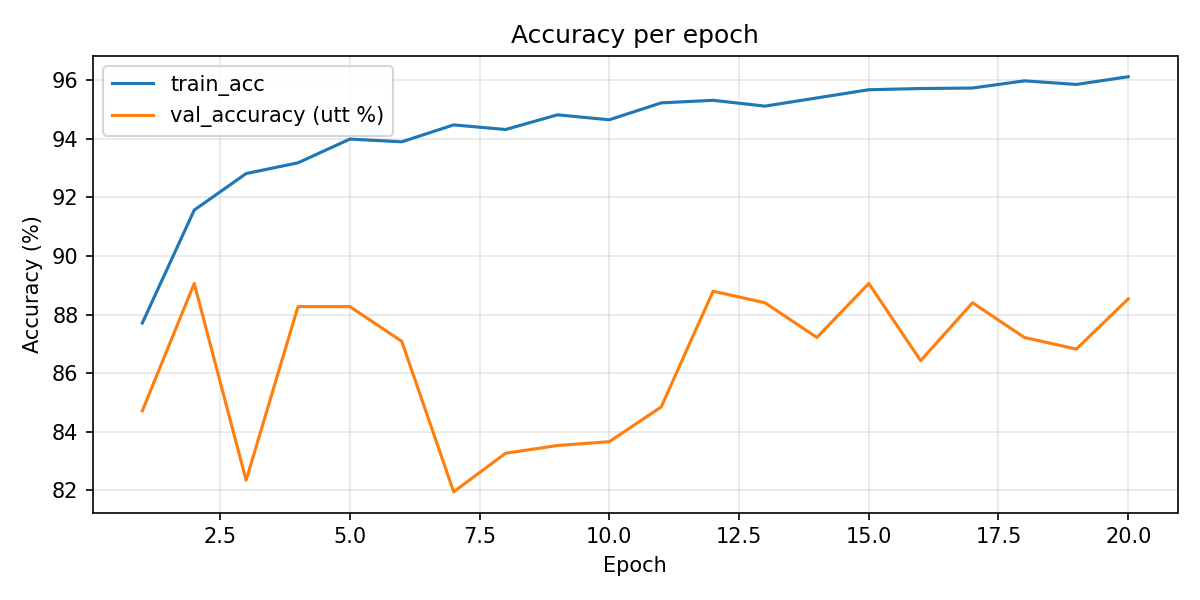
\includegraphics[width=\linewidth]{reduced_ft_acc.png}
  \caption{Accuracy}
\end{subfigure}
\caption{Reduced --- LibriSpeech fine-tuning (20 epochs).}
\end{figure}

\subsection{Filter interpretability after TIMIT}

Figures~\ref{fig:reduced-analysis}--\ref{fig:reduced-tsne-qf} show the frozen triangular bank after TIMIT retraining: accumulative magnitude coverage, center-frequency histogram, gender-balanced t-SNE ($n{=}2000$ male / $2000$ female chunks), and quality factor $Q=f_c/B$.

\begin{figure}[H]
\centering
\begin{subfigure}[t]{0.48\textwidth}
  \centering
  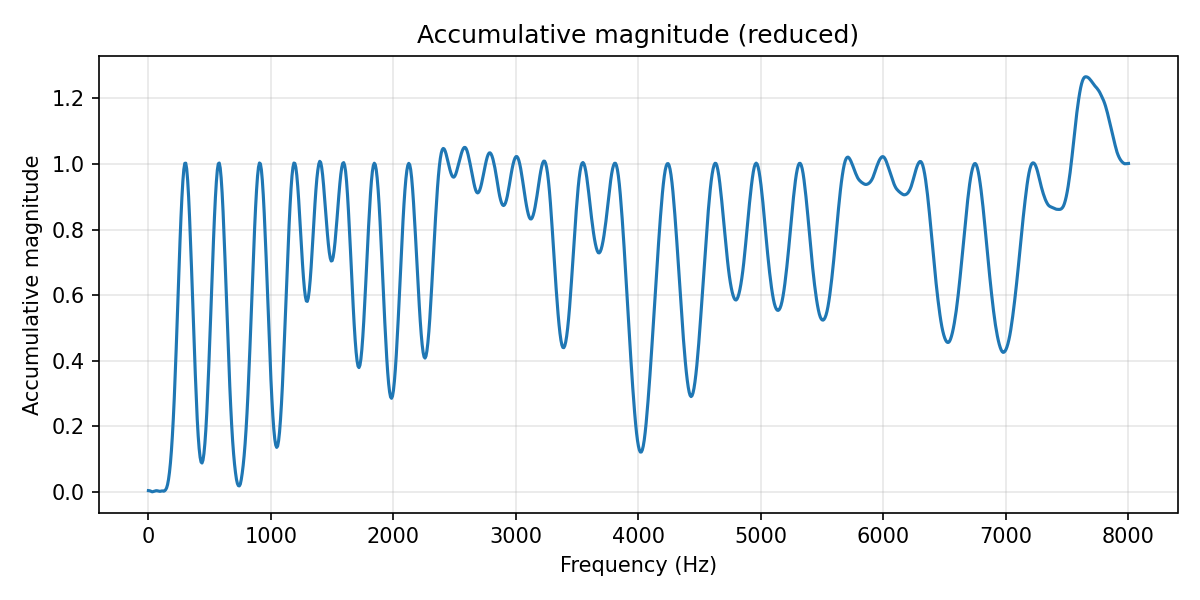
\includegraphics[width=\linewidth]{reduced_accum_mag.png}
  \caption{Accumulative magnitude}
\end{subfigure}\hfill
\begin{subfigure}[t]{0.48\textwidth}
  \centering
  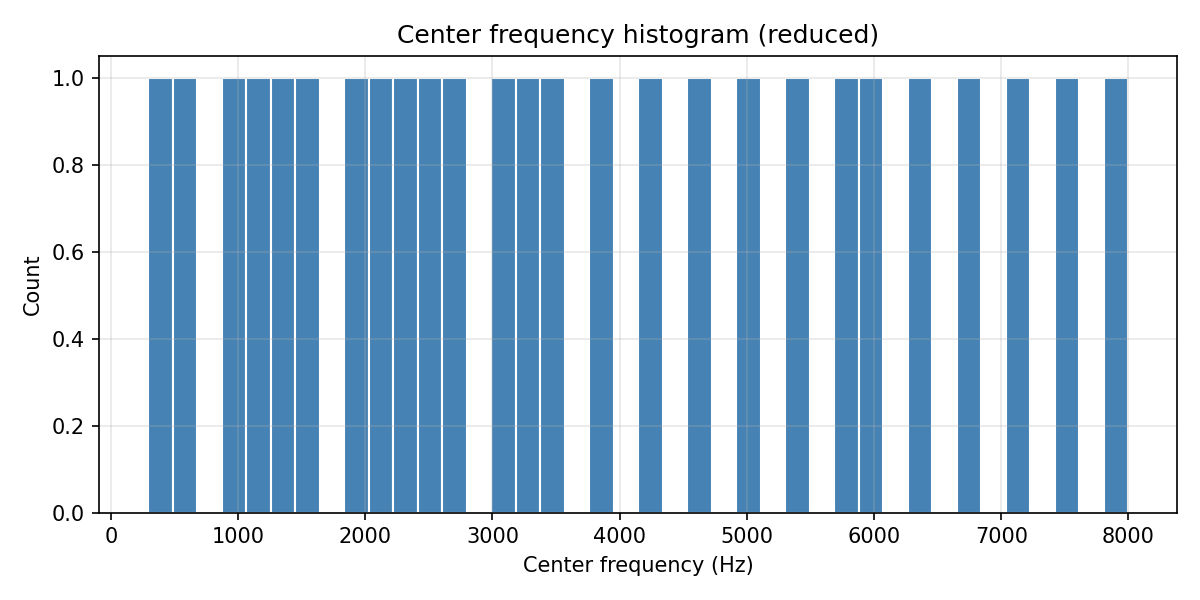
\includegraphics[width=\linewidth]{reduced_fc_hist.png}
  \caption{Center-frequency histogram}
\end{subfigure}
\caption{Reduced filter-bank analysis after TIMIT retraining.}
\label{fig:reduced-analysis}
\end{figure}

\begin{figure}[H]
\centering
\begin{subfigure}[t]{0.48\textwidth}
  \centering
  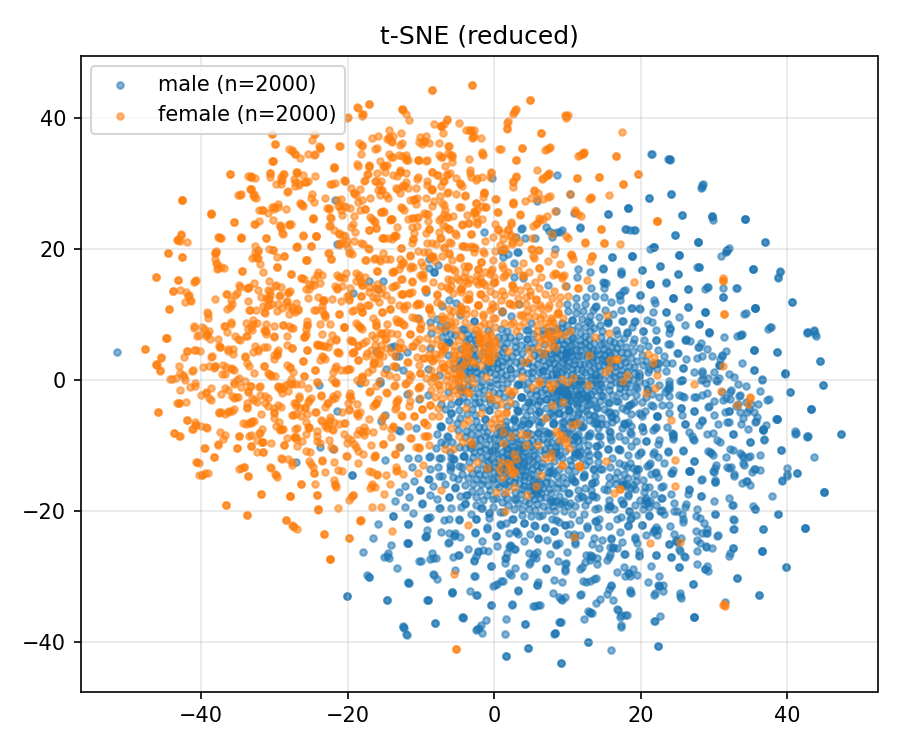
\includegraphics[width=\linewidth]{reduced_tsne.png}
  \caption{t-SNE (TIMIT test, balanced)}
\end{subfigure}\hfill
\begin{subfigure}[t]{0.48\textwidth}
  \centering
  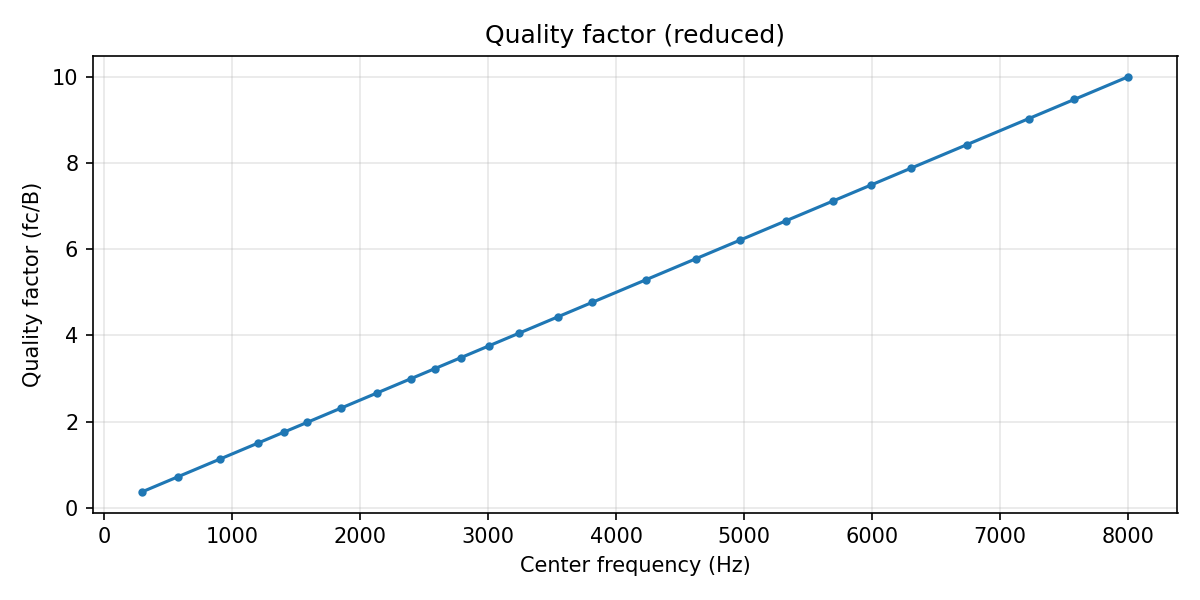
\includegraphics[width=\linewidth]{reduced_qf.png}
  \caption{Quality factor $Q{=}f_c/B$}
\end{subfigure}
\caption{Reduced: feature separability and quality-factor profile (TIMIT).}
\label{fig:reduced-tsne-qf}
\end{figure}

\subsection{Filter interpretability after fine-tuning (RAVDESS)}

After LibriSpeech fine-tuning, the same frozen frontend is analyzed on RAVDESS features (Fig.~\ref{fig:reduced-ft-analysis}--\ref{fig:reduced-ft-tsne-qf}). Magnitude / $f_c$ structure is essentially unchanged (Conv1 frozen); t-SNE still separates male and female under emotional speech, consistent with the $90.83\%$ RAVDESS accuracy.

\begin{figure}[H]
\centering
\begin{subfigure}[t]{0.48\textwidth}
  \centering
  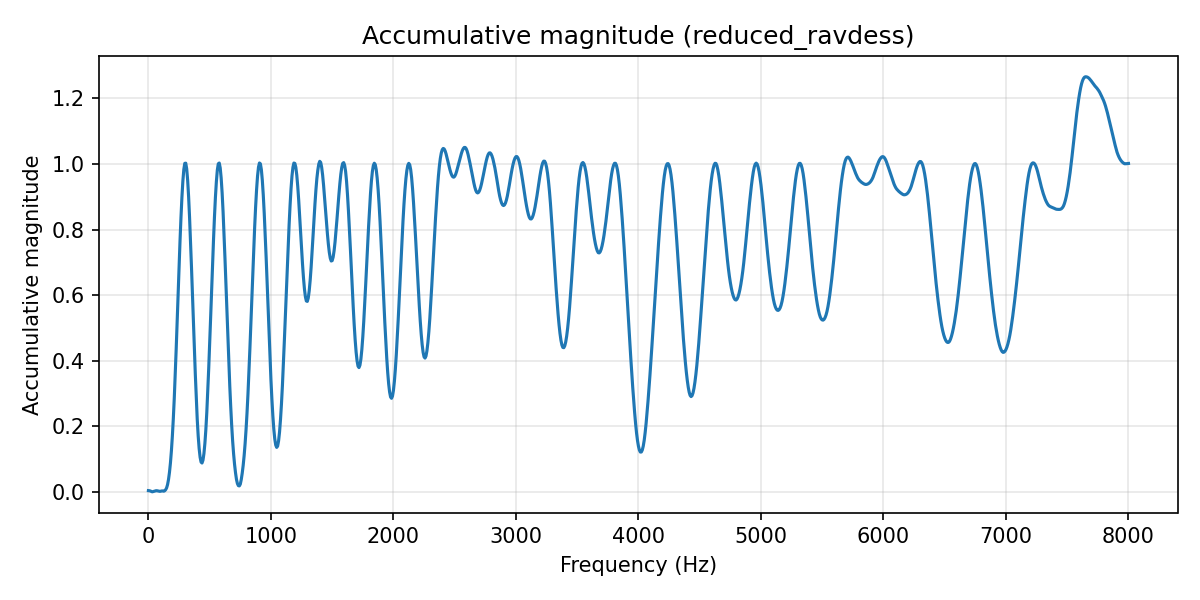
\includegraphics[width=\linewidth]{reduced_ft_accum_mag.png}
  \caption{Accumulative magnitude}
\end{subfigure}\hfill
\begin{subfigure}[t]{0.48\textwidth}
  \centering
  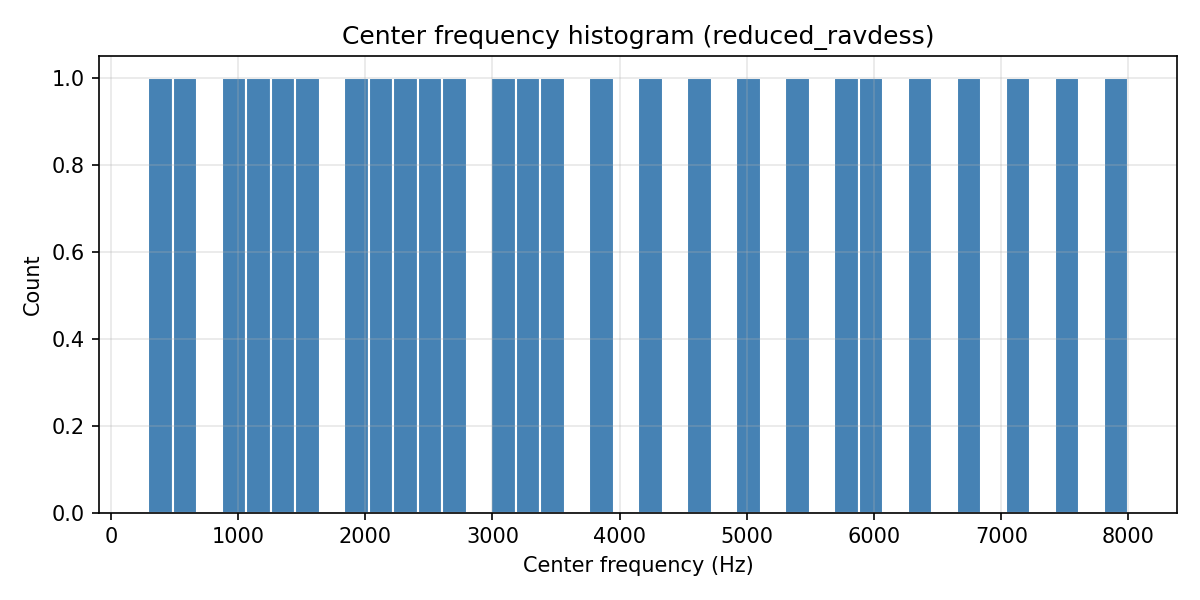
\includegraphics[width=\linewidth]{reduced_ft_fc_hist.png}
  \caption{Center-frequency histogram}
\end{subfigure}
\caption{Reduced filter-bank analysis after fine-tuning (RAVDESS eval features).}
\label{fig:reduced-ft-analysis}
\end{figure}

\begin{figure}[H]
\centering
\begin{subfigure}[t]{0.48\textwidth}
  \centering
  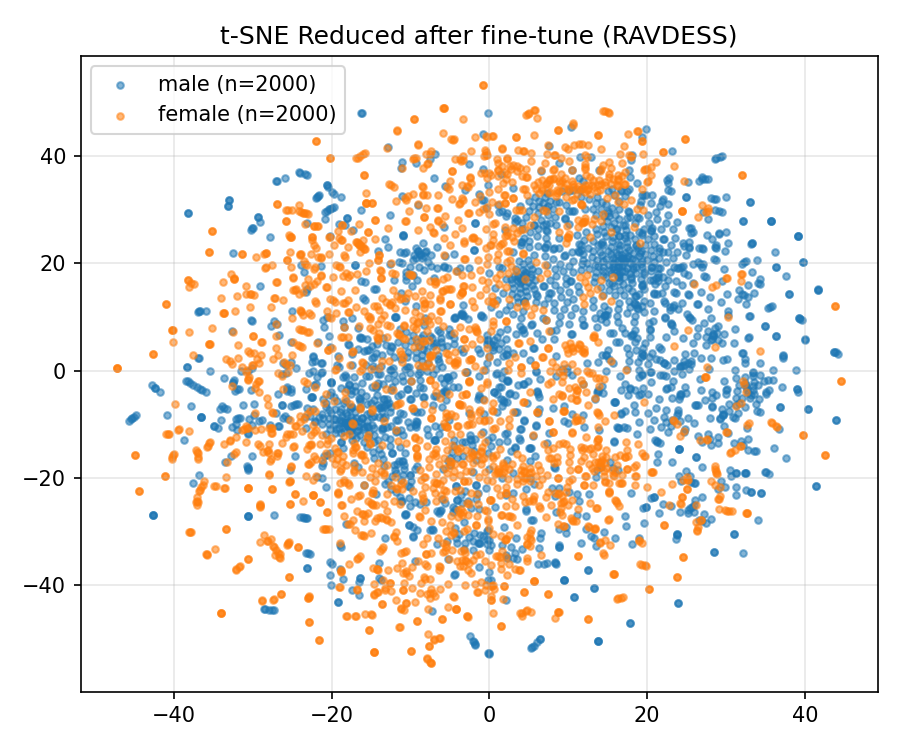
\includegraphics[width=\linewidth]{reduced_ft_tsne.png}
  \caption{t-SNE (RAVDESS, balanced)}
\end{subfigure}\hfill
\begin{subfigure}[t]{0.48\textwidth}
  \centering
  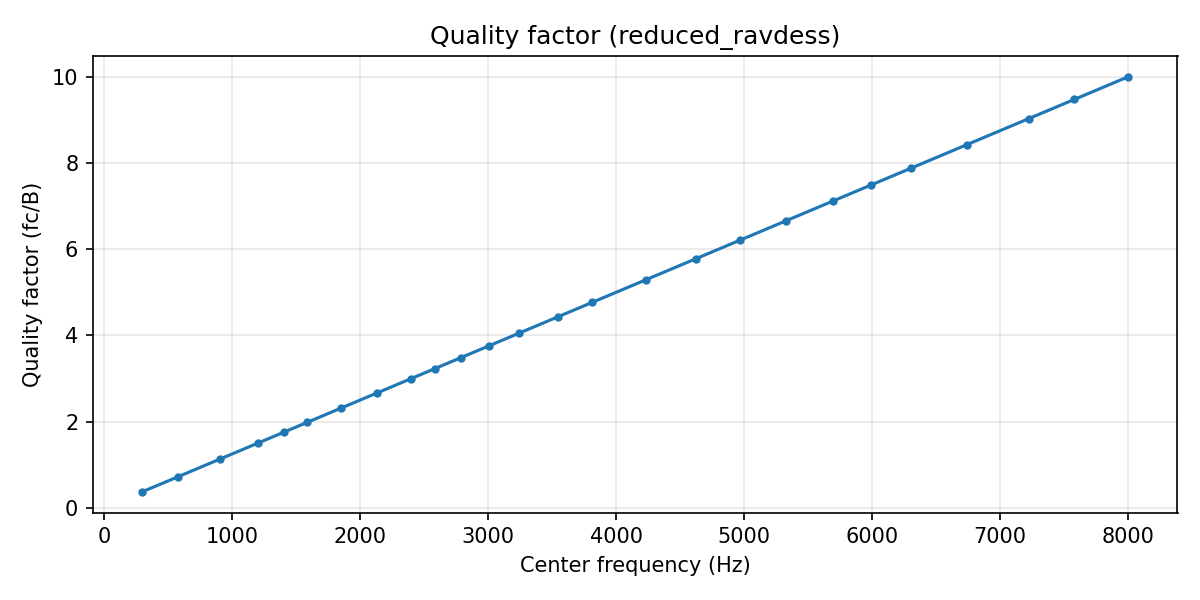
\includegraphics[width=\linewidth]{reduced_ft_qf.png}
  \caption{Quality factor $Q{=}f_c/B$}
\end{subfigure}
\caption{Reduced after fine-tuning: RAVDESS feature separability and $Q$-profile.}
\label{fig:reduced-ft-tsne-qf}
\end{figure}

% ============================================================
\section{Discussion of Discrepancies}
\label{sec:discussion}
% ============================================================

\subsection{Why TIMIT results align closely}

TIMIT is clean, studio-quality speech with limited acoustic variability. Under these conditions, even a 50-epoch schedule with random chunk sampling is sufficient for AFM frontends to approach the asymptotic accuracy of the paper. The residual differences of a few tenths of a percent are consistent with (i)~single-run noise versus three-run averaging and (ii)~incomplete convergence relative to 500 epochs.

\subsection{Why RAVDESS and VoxCeleb gaps are larger}

Out-of-domain corpora stress robustness to emotion (RAVDESS), channel, and speaker diversity (VoxCeleb). We identify five primary factors:

\begin{enumerate}[leftmargin=1.6em,itemsep=0.4em]
  \item \textbf{Fine-tuning duration.} The paper adapts for 200 epochs; we use 20 ($10\times$ shorter). Domain adaptation for unconstrained Free-CNN appears especially sensitive to this budget (largest deficits in Tables~\ref{tab:ravdess}--\ref{tab:vox}).
  \item \textbf{Fine-tuning corpus scale.} \texttt{train-clean-360} covers $\approx$921 speakers; \texttt{dev-clean} covers $\approx$40. The reduced speaker diversity limits the transferable gender cues acquired during fine-tuning.
  \item \textbf{VoxCeleb evaluation set.} Paper numbers are for full VoxCeleb1; ours are for the official test partition only. Absolute accuracy is therefore not strictly comparable, though relative ranking among frontends remains informative.
  \item \textbf{Single-run reporting.} Published tables average three seeds; we report one seed (42). Run-to-run variance of order $0.1$--$0.5$\,pp is plausible on TIMIT and larger on OOD sets.
  \item \textbf{Stochastic training coverage.} Eight random chunks per utterance per epoch under-samples long utterances relative to exhaustive 10\,ms hopping, which may slightly weaken low-SNR or boundary-frame robustness.
\end{enumerate}

\subsection{Positive observations}

Despite these constraints, AFM frontends remain competitive:
\begin{itemize}[leftmargin=1.6em,itemsep=0.25em]
  \item Sinc2 and Reduced recover within $1.2$--$2.2$\,pp of the paper on VoxCeleb1-test;
  \item Gauss slightly exceeds the paper on RAVDESS;
  \item Reduced achieves the best TIMIT CER with only 26 frozen filters, supporting the paper's claim that pole clustering yields a compact yet accurate bank.
\end{itemize}

% ============================================================
\section{Conclusion}
% ============================================================

We have reproduced the AFM-frontend speaker gender recognition pipeline of Fayyazi and Shekofteh (2023), spanning TIMIT training, Cascade pole reduction, LibriSpeech fine-tuning, and OOD evaluation on RAVDESS and VoxCeleb1-test. In-domain TIMIT results closely match the published means. Out-of-domain accuracy is lower, for reasons that are largely attributable to controlled protocol differences (epoch budget, fine-tuning data scale, and evaluation subset) rather than to an architectural failure of the AFM approach. The accompanying figures---training curves, complex-plane pole reduction, and filter interpretability analyses---document that the Reduced bank preserves discriminative spectral coverage with far fewer parameters, in line with the paper's central thesis.

\paragraph{Future work.}
Closing the OOD gap would require (i)~fine-tuning on LibriSpeech \texttt{train-clean-360} for $\ge$200 epochs, (ii)~evaluation on full VoxCeleb1, and (iii)~three independent runs with mean$\pm$std reporting as in the original study.

% ============================================================
\begin{thebibliography}{9}

\bibitem{fayyazi2023}
H.~Fayyazi and Y.~Shekofteh,
``Exploiting auditory filter models as interpretable convolutional frontends to obtain optimal architectures for speaker gender recognition,''
\emph{Applied Acoustics}, vol.~213, Art.~109635, 2023.

\bibitem{ravanelli2018}
M.~Ravanelli and Y.~Bengio,
``Speaker recognition from raw waveform with SincNet,''
in \emph{Proc.\ IEEE SLT}, 2018, pp.~1021--1028.

\bibitem{garofolo1993}
J.~S.~Garofolo et~al.,
``TIMIT acoustic-phonetic continuous speech corpus,''
LDC93S1, Linguistic Data Consortium, 1993.

\bibitem{panayotov2015}
V.~Panayotov, G.~Chen, D.~Povey, and S.~Khudanpur,
``LibriSpeech: An ASR corpus based on public domain audio books,''
in \emph{Proc.\ IEEE ICASSP}, 2015, pp.~5206--5210.

\bibitem{livingstone2018}
S.~R.~Livingstone and F.~A.~Russo,
``The Ryerson Audio-Visual Database of Emotional Speech and Song (RAVDESS),''
\emph{PLoS ONE}, vol.~13, no.~5, e0196391, 2018.

\bibitem{nagrani2017}
A.~Nagrani, J.~S.~Chung, and A.~Zisserman,
``VoxCeleb: A large-scale speaker identification dataset,''
in \emph{Proc.\ Interspeech}, 2017, pp.~2616--2620.

\end{thebibliography}

% ============================================================
\appendix
\section{Additional TIMIT Training Curves}
% ============================================================

\begin{figure}[H]
\centering
\begin{subfigure}[t]{0.48\textwidth}
  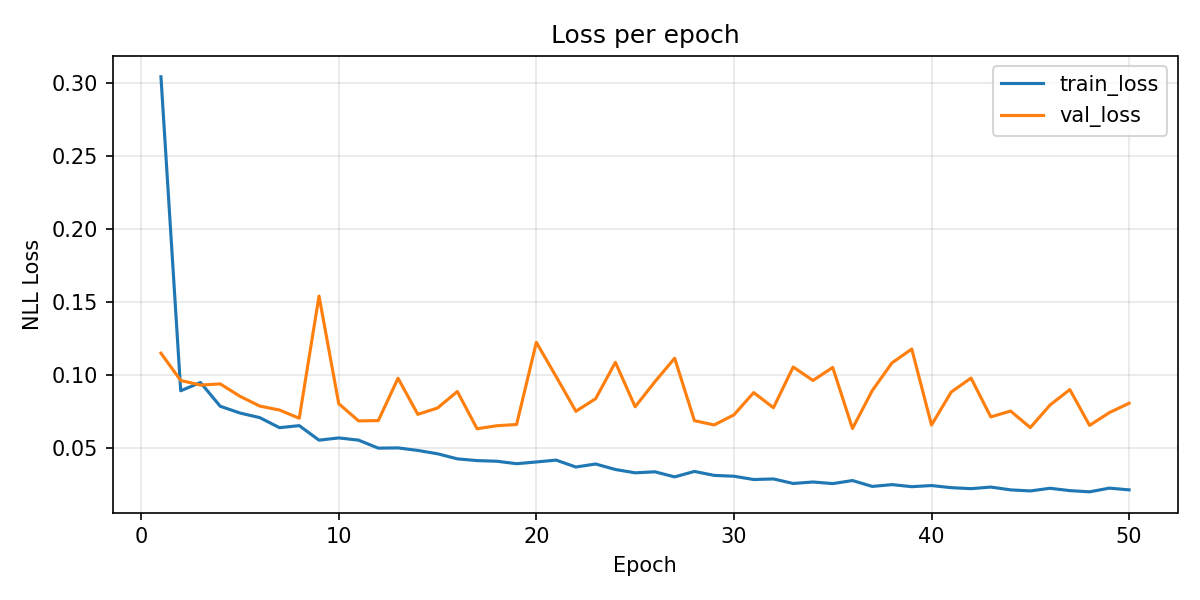
\includegraphics[width=\linewidth]{sinc_timit_loss.png}
\end{subfigure}\hfill
\begin{subfigure}[t]{0.48\textwidth}
  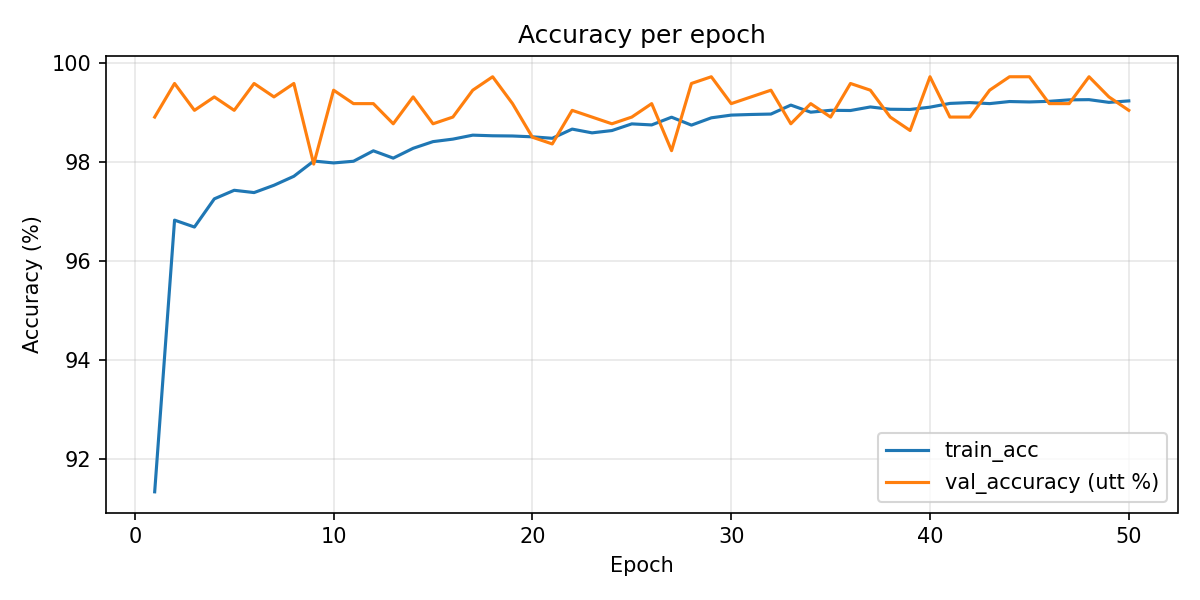
\includegraphics[width=\linewidth]{sinc_timit_acc.png}
\end{subfigure}
\caption{Sinc --- TIMIT training.}
\end{figure}

\begin{figure}[H]
\centering
\begin{subfigure}[t]{0.48\textwidth}
  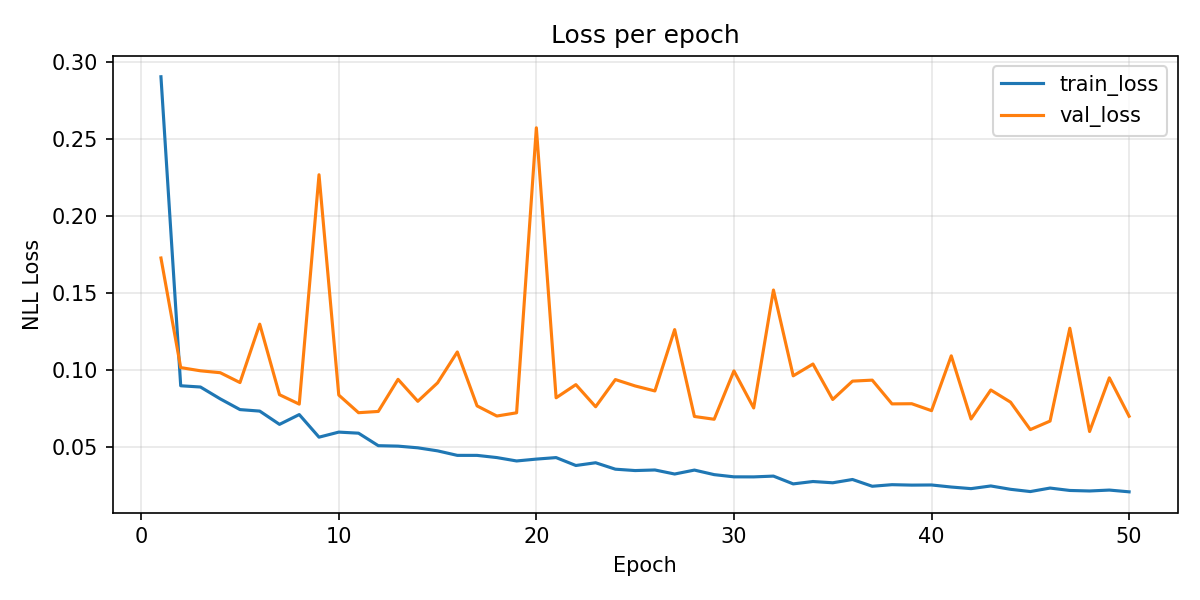
\includegraphics[width=\linewidth]{sinc2_timit_loss.png}
\end{subfigure}\hfill
\begin{subfigure}[t]{0.48\textwidth}
  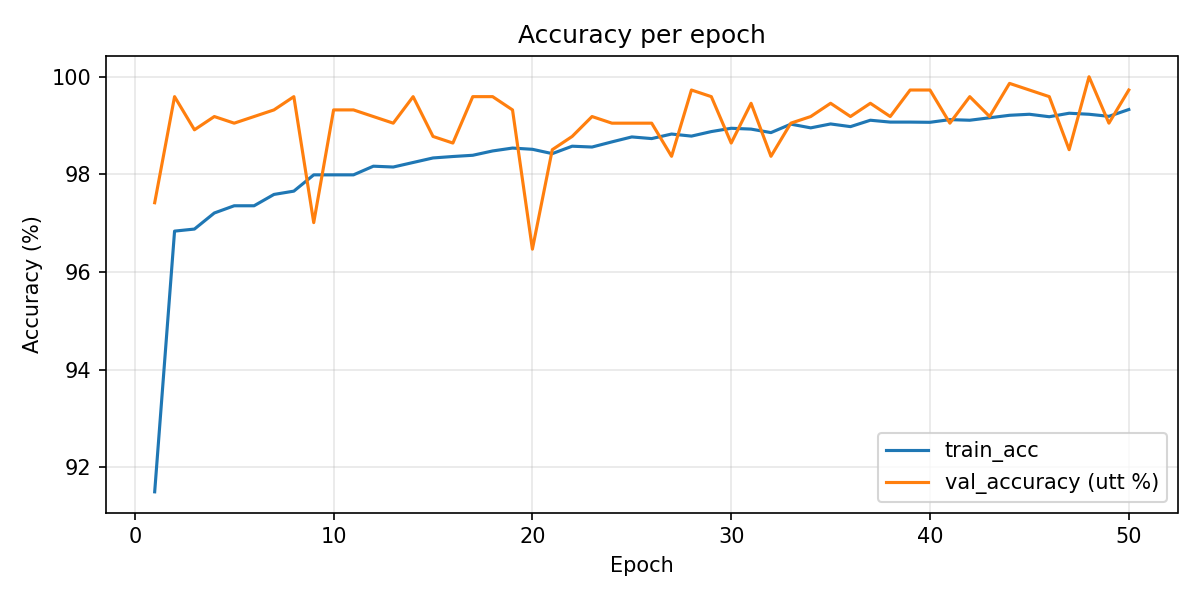
\includegraphics[width=\linewidth]{sinc2_timit_acc.png}
\end{subfigure}
\caption{Sinc2 --- TIMIT training.}
\end{figure}

\begin{figure}[H]
\centering
\begin{subfigure}[t]{0.48\textwidth}
  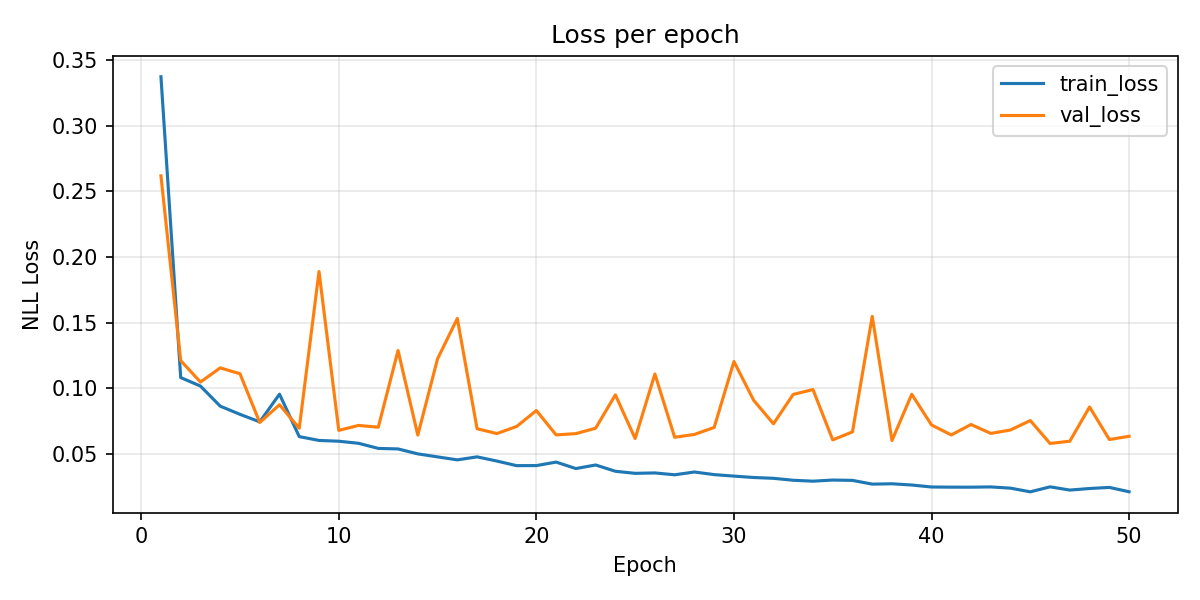
\includegraphics[width=\linewidth]{gamma_timit_loss.png}
\end{subfigure}\hfill
\begin{subfigure}[t]{0.48\textwidth}
  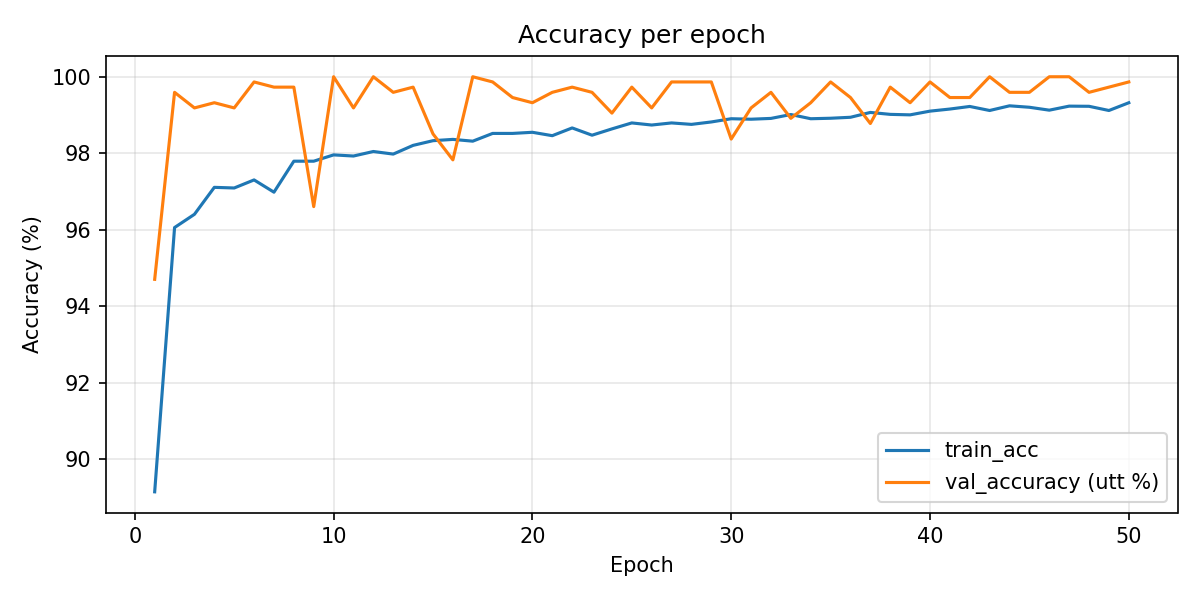
\includegraphics[width=\linewidth]{gamma_timit_acc.png}
\end{subfigure}
\caption{Gamma --- TIMIT training.}
\end{figure}

\begin{figure}[H]
\centering
\begin{subfigure}[t]{0.48\textwidth}
  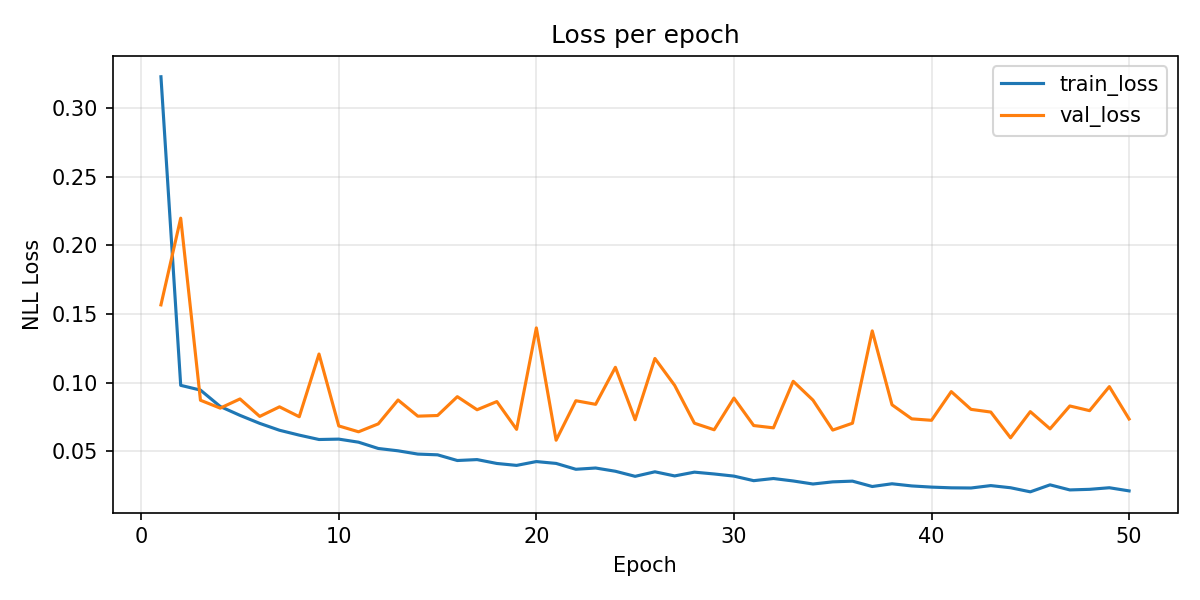
\includegraphics[width=\linewidth]{gauss_timit_loss.png}
\end{subfigure}\hfill
\begin{subfigure}[t]{0.48\textwidth}
  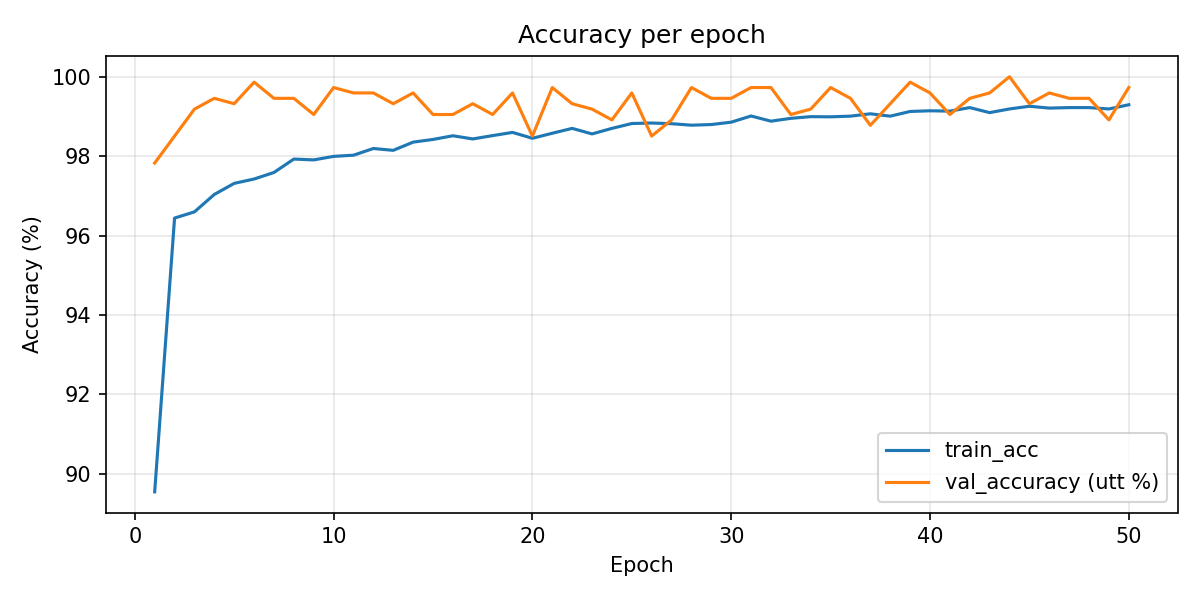
\includegraphics[width=\linewidth]{gauss_timit_acc.png}
\end{subfigure}
\caption{Gauss --- TIMIT training.}
\end{figure}

\begin{figure}[H]
\centering
\begin{subfigure}[t]{0.48\textwidth}
  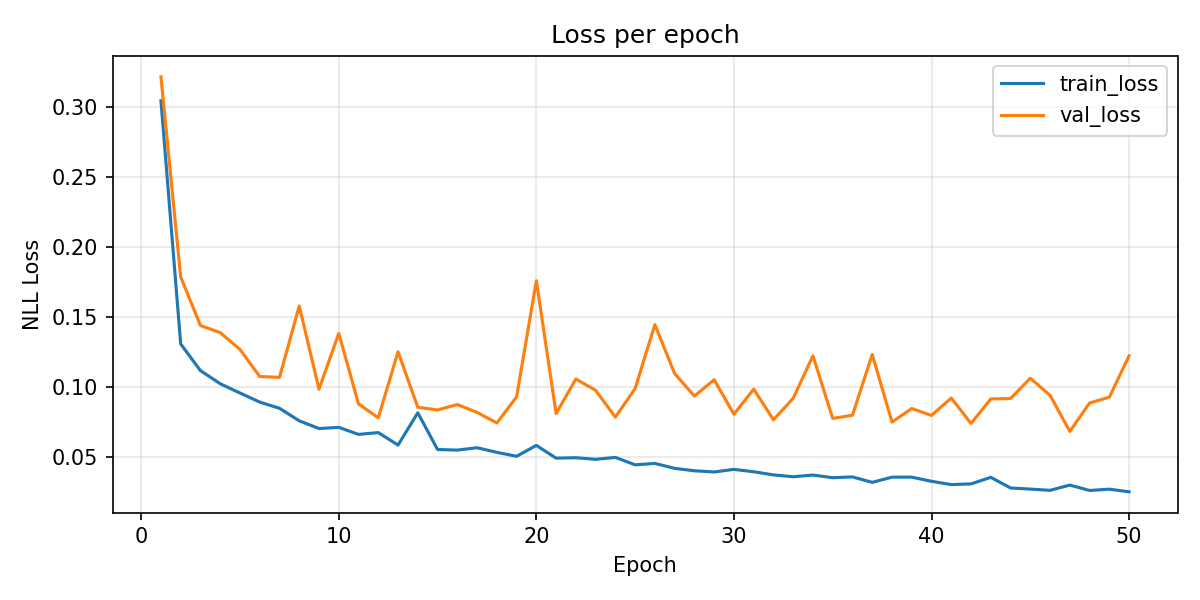
\includegraphics[width=\linewidth]{free_timit_loss.png}
\end{subfigure}\hfill
\begin{subfigure}[t]{0.48\textwidth}
  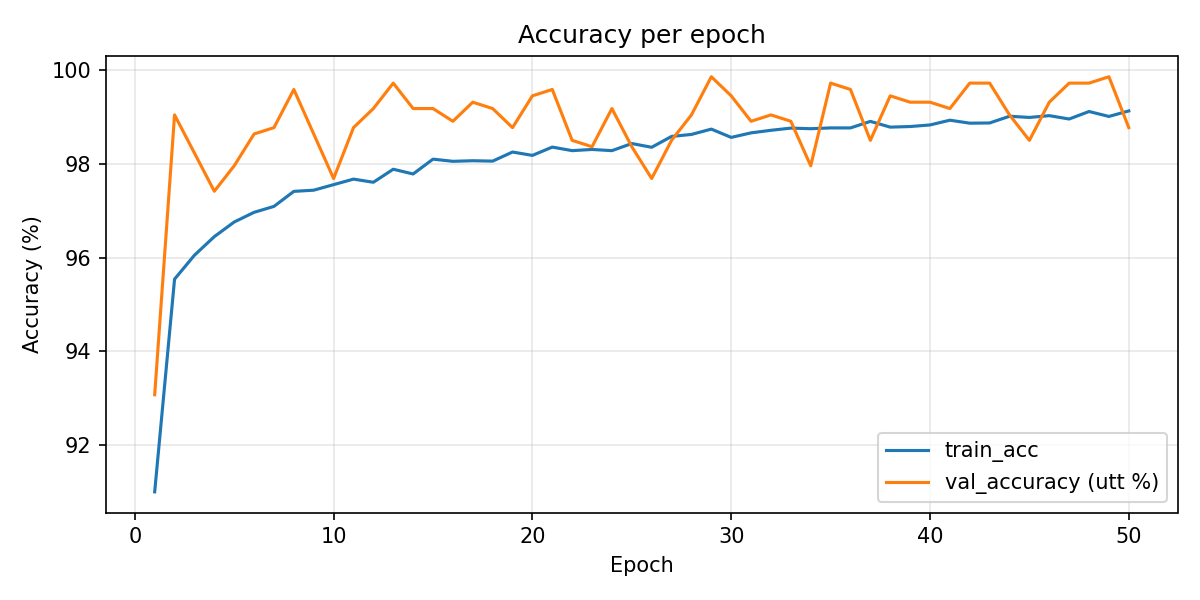
\includegraphics[width=\linewidth]{free_timit_acc.png}
\end{subfigure}
\caption{Free-CNN --- TIMIT training.}
\end{figure}

\end{document}
